\documentclass[12pt,headsepline,a4paper]{scrartcl}
%\usepackage[]{graphicx}
\usepackage{lmodern}
\usepackage{float}
\usepackage{graphicx}
\usepackage{booktabs} 
\usepackage[OT2,T1]{fontenc}
\usepackage[utf8]{inputenc}
\usepackage[russian,ngerman]{babel}
%\usepackage[style=authoryear-icomp,backend=bibtex,maxnames=2]{biblatex}
\usepackage[babel,german=guillemets]{csquotes}
\usepackage{paralist} 
\usepackage{multirow}
\usepackage{tabularx}
\usepackage{amsfonts}
\usepackage[
backend = bibtex8,
bibencoding = utf8,
defernumbers=true,
natbib = true,
style = authoryear-icomp, 
maxnames = 2,
minnames = 1,
backref = true,
backrefstyle = two, 
]{biblatex} 
\addbibresource{ba-thesis.bib}
\usepackage{qtree}
%\usepackage[options]{algorithm2e}
\usepackage{algpseudocode}
\usepackage{algorithm}
%\renewcommand\ttdefault{lmtt}
\usepackage{fancyvrb}
%\bibliography{syll_lit}  
%\usepackage[german]{varioref}
%\usepackage{bibgerm}  
%\usepackage{natbib} 
\usepackage{tipa} 
\usepackage[german]{fancyref} 
\usepackage{caption}
\newcommand\textcyr[1]{{\fontencoding{OT2}\fontfamily{wncyr}\selectfont #1}}
\usepackage{microtype} 
\usepackage[onehalfspacing]{setspace}
\usepackage[paper=a4paper,margin=1in]{geometry}
%\usepackage[a4paper]{geometry}
%\geometry{left=4.5cm,right=2cm,top=2cm, bottom=2cm}
\usepackage{tikz}
\newcommand\labialized[2][]{\tikz[overlay]\node[draw=black,inner sep=2pt, anchor=text, rectangle,rounded corners=2mm,#1] {#2};\phantom{#2}}
%\newcommand\autocite[1]{\cite}
%\DeclareNameFormat{labelname}{\textsc{#1}}
\usepackage{scrpage2}  %<---
\pagestyle{scrheadings}%<
\clearscrheadfoot

\chead{\leftmark}
\automark[section]{section} 
\rohead{\pagemark}

\begin{document}
\begin{titlepage}
\date{}
\author{}

 
%\textsc{\Large Vergleich der Silbenmodelle des Russischen mit Hilfe eines Natural Language Processing-Ansatzes}\\[0.5cm]

% \normalsize{
\title{\Large Vergleich der Silbenmodelle des Russischen mit Hilfe eines Natural Language Processing-Ansatzes}
{\let\newpage\relax\maketitle}


\begin{center}
Wissenschaftliche Hausarbeit\\
zur Erlangung des akademischen Grades\\
Bachelor of Arts (B.A.)\\
der Universität Hamburg
\end{center}
\vfill
\begin{center}
vorgelegt von\\
Igor Fischer\\
geboren in\\
Temirtau (Kasachstan)
\null
\vfill
\noindent
Hamburg 2014
\end{center}

\pagenumbering{gobble}
\end{titlepage}
\newgeometry{left=4.5cm,right=2cm,top=2cm, bottom=2cm}
%\pagestyle{headings}\makeatletter
%\setcounter{page}{1}

\tableofcontents
\thispagestyle{empty}
% 
% \begingroup
% %\fontencoding{OT2}\fontfamily{wncyr}\fontsize{10pt}{12pt}\selectfont
% \begin{figure}
% \centering
% 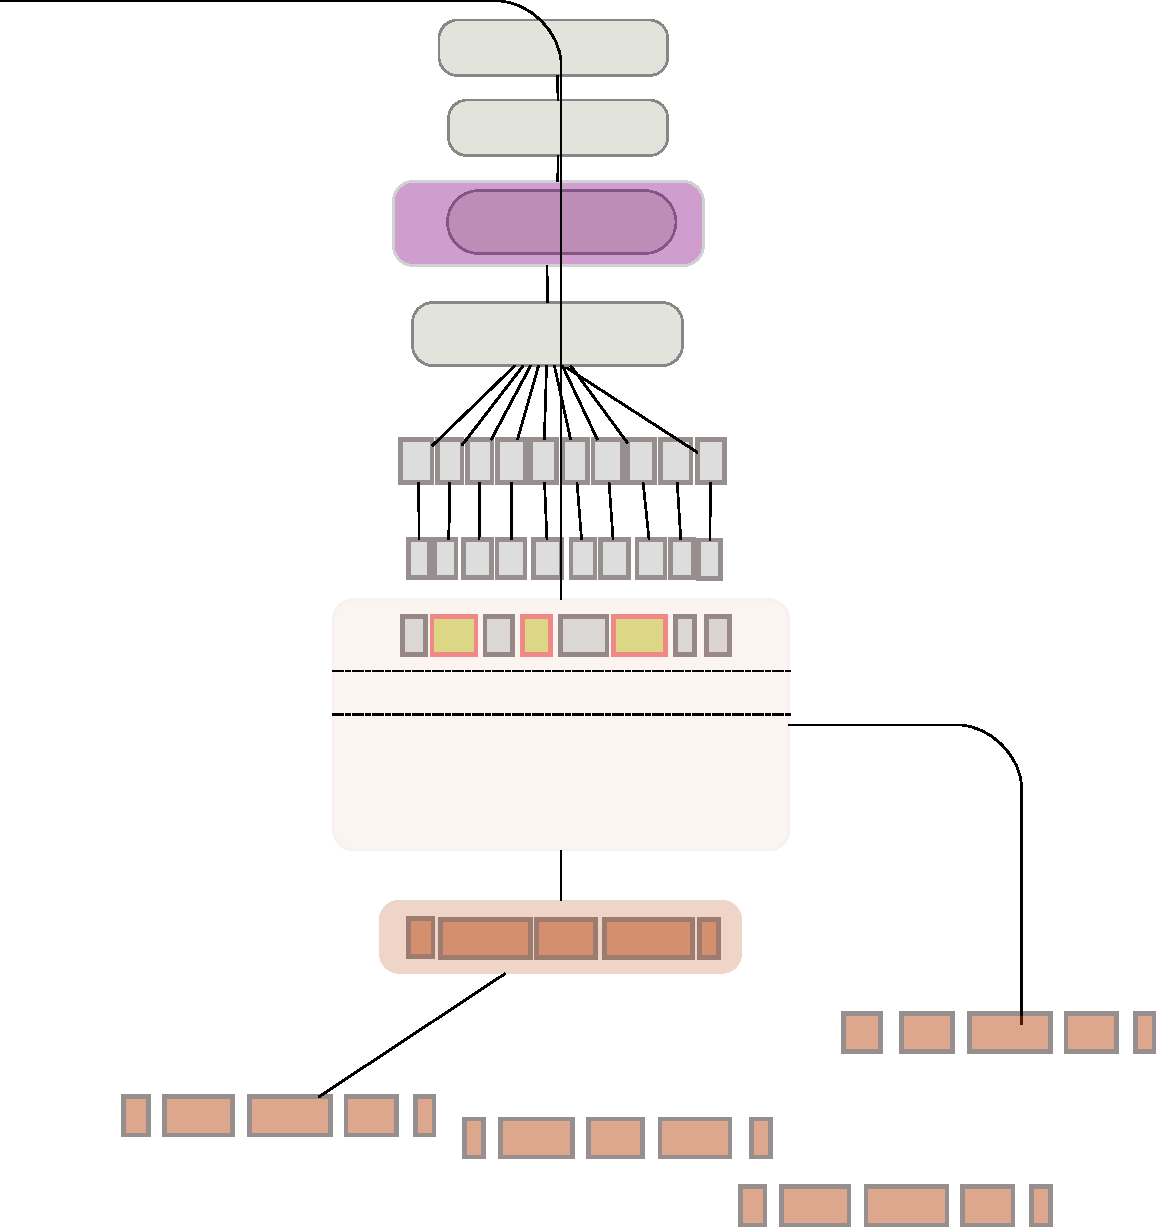
\includegraphics{figures/syllaru_system.pdf}
% \end{figure}
% \endgroup
% 
% \begin{figure}
% \centering
% \def\svgwidth{\columnwidth}
% \input{figures/freq_map.pdf_tex}
% \end{figure}
% 
\section*{Einleitung}
\markboth{Einleitung}{Einleitung}
\addcontentsline{toc}{section}{Einleitung}
\pagenumbering{arabic}
"`Syllables govern the world"', sagte einmal der irisch-britische Schriftsteller George B. Shaw. Auch wenn er damit wohl die Macht von Wörtern beschreiben wollte, hat er doch zwei Tatsachen ausgedrückt: Wörter bestehen aus Silben und Silbe als Begriff ist nicht nur für akademische Kreise reserviert. \textcite[164]{gold2011} schreibt zur Rolle in der Lingustik: "`The syllable is one of the oldest constructs in the study of language, and most studies of phonology have found a place for the syllable within them."' Trotz der langen Geschichte bleibt der Begriff umstritten. In der Russistik gibt es zumindest 3 rein russistische Silbenmodelle. An der Theorie fehlt es allerdings nicht, aber an der Computerisierung.

Die vorliegende Arbeit soll einen Beitrag zum Aufheben dieses Umstandes leisten. Tatsächlich soll nicht noch ein theoretischer Beitrag zur Silbe geleistet werden, sondern die Russistik um einen praktischen Ansatz bereichert werden. Die konkreten Subziele sind zum einen, dem Forscher die Wahl zu lassen, unter welchem Modell er einen Text oder eine Aufgabe betrachten will. Andererseits soll alles leicht modulierbar und ergänzbar sein, damit der Forscher die Anwendung seinen Zielen anpassen kann.

Dies soll mit einem hier entwickelten Programm erreicht werden. Dieses soll aus state-of-art Elementen geschaffen sein, die es mittelfristig zu mehr machen können als einer Momentaufnahme. Zum einen wird Python als Sprache verwendet, die in Data Science und akademischer Welt sehr erfolgreich ist. Zum anderen basiert das Programm auf pandas, einer Programmbibliothek für Python. Dieses Projekt von 2008 ist mit 5 Jahren sehr jung, doch in Kombination mit Python macht es durch die Zugänglichkeit anderen Programmierprachen wie R, SAS oder C++ in der Finanzindustrie bereits jetzt Konkurrenz: "`Institutions have found that Python is well-suited both
as an interactive analysis environment as well as enabling robust systems to be developed
often in a fraction of the time it would have taken in Java or C++"'\autocite[329]{mckinney2012}. Python ist nicht zuletzt prädestiniert für sprachliche Aufgaben durch andere Bibliotheken wie NLTK (Natural Language Toolkit) oder scikit-learn (Machine-Learning-Algorithmen).

Die Struktur dieser Arbeit spiegelt auch die Etappen der Entwicklung des Programms wider: Zunächst sollen in Kapitel \ref{sec:theor_nlp} bestimmte Rahmenbedingungen und nützliche Begriffe geklärt werden. Dies ist der kürzeste Teil der Arbeit, soll aber durch seine Kürze der Absicht der Arbeit dienen, die Silbe sehr praktisch zu untersuchen. Anders ausgedrückt: Theorie soll nur so weit einfließen, wie es für die Umsetzung und Verständnis des Programms notwendig ist. 

Kapitel \ref{sec:sylmodels} bietet eine kurze Vorstellung der behandelten Silbenmodelle und stellt ebenfalls die notwendigste Theorie vor, um sie zu verstehen. Zu keinem Zeitpunkt soll ein Modell dem anderen bevorzugt werden, höchstens Umstände thematisiert werden, die eine Implementierung schwierig machen.

In Kapitel \ref{sec:mate_meth} soll diese theoretische Grundlage der Silbe mit einer technischen Grundlage der Algorithmen angereichert werden. Hier soll ebenfalls ein wichtige Zwischenstation des Programms erklärt werden, nämlich die Transkription hin  zur Lautebene. Da dies für genaue Silbenstatistiken sehr wichtig ist, wurde hier besonders viel Arbeit investiert. Der Verfasser zählt dies ebenfalls als wichtige Leistung der vorliegenden Arbeit. Ausgehend von der "`Heimat"' dieser Arbeit (die Linguistik), soll die Code- und Mathematik-Seite in den Hintergrund rücken und eher durch Pseudocode und Abbildungen abstrahiert dargestellt werden.

Das Kapitel \ref{sec: stat_tst} zur statistischen Auswertung soll den Leser für einige Probleme sensibilisieren, die mit den Daten verbunden sind. Das ist wichtig, da das Programm prinzipiell jedem ermöglichen soll, eine Auswertung vorzunehmen, die Daten aber tückisch sein können. Gleichzeitig sollen aber einige Vorschläge  gemacht werden, um die Probleme zu lösen. Es soll eine Technik Anwendung finden, die sich sehr gut für diese Art von Daten eignet.

\subsection*{Formales}
Im Grunde folgt die Arbeit den Konventionen üblicher Arbeiten. Betonte Wörter werden kursiv geschrieben, ebenfalls auch neu eingeführte Konzepte. Da die Software und die Literatur zu einem Großteil Englisch ist, folgt die Arbeit angelsächsischen Konventionen in Bezug auf Zahlen: Dezimaltrenner "`."', Tausendertrennzeichen "`,"', wobei der letztere nur bei $\geq$5 Zahlen Anwendung findet.
 
Der oft gemachte Unterschied zwischen Tokens und Types soll kurz an einem Beispiel veranschaulicht werden: Nehmen wir eine Aufzählung [a,b,a,a,b,c]. In ihr finden sich 6 Tokens, aber nur 3 Types \{a,b,c\}, gleichzeitig entspricht \{a,b,c\} dem Set von der Aufzählung. Dieser wichtige Unterschied soll in dieser Arbeit häufig gemacht werden.

Es finden sich größtenteils Beispiele, die nicht in IPA-Umschrift sind. Sie wird nur verwendet, wenn tatsächlich ein für Silbengrenzen wichtiger Unterschied zwischen Graphemen und Lauten herrscht. Der Grund ist einfach: Das Programm arbeitet zu keiner Zeit mit der IPA, sondern mit einer pseudokyrillischen Form (\textcyr{што, мяхкий, чуство}), die in eine spezielle Form von SAMPA\footnote{http://www.phon.ucl.ac.uk/home/sampa/russian.htm} übertragen wird. Die Argumente dafür werden im Laufe der Arbeit vorgestellt.

\newpage

\section{Theoretische Grundlagen zur Silbe und NLP}
\label{sec:theor_nlp}

\subsection{Silbentermini}
Die grundlegenden Silbenbegriffe sollen hier in Anlehnung an \textcite[5--10]{duan2009} wiedergegeben werden. Eine Silbe besteht immer aus einem \textit{Nucleus}, im Russischen ist es immer ein Vokal, in anderen Sprachen können Sonore diese Rolle einnehmen wie im Englischen oder Italienischen \autocite{iaco2011}. Die Konsonanten vor einem Nucleus nennt man \textit{Onsets}, die Konsonanten nach dem Vokal bilden die \textit{Coda}. Coda und Nucleus bilden zusammen die Gruppe namens \textit{Reim} (rime oder rhyme im Englischen), trivialerweise weil dieser Teil für Reime in den Sprachen verantwortlich ist. Einfache Onsets und Codas bestehen aus einem Konsonanten wie in \fref{fig: sim_syll} (a), komplexe haben mehrere (\fref{fig: sim_syll}(b)). Die ganze Silbe wird mit dem griechischen Buchstaben $\sigma$ "`Sigma"' bezeichnet.
Die ersten beiden Strukturen bilden \textit{geschlossene Silben} ab, da die Silbe mit einem Konsonanten endet, Beispiel (c) bildet dagegen eine \textit{offene Silbe} ab. Das Silbenskelett bezieht sich auf die Kategorien Konsonant und Vokal. Erstes Beispiel hat ein Silbenskelett CVC, (b) CCVC, (c) CV.
 
\begin{figure}[htbp]
\parbox[t]{0.3\textwidth}{ (a)~\Tree 
 	[.$\sigma$ [.Onset d ] [.Reim [.Nucleus \textipa{1} ] 	[.Coda m ]]] }
\parbox[t]{0.3\textwidth}{ (b)~\Tree 
   [.$\sigma$ [.Onset st ] [.Reim [.Nucleus \textipa{O} ] [.Coda \textipa{\textsuperimposetilde{l}} ]]] }
\parbox[t]{0.3\textwidth}{ (c)~\Tree 
   [.$\sigma$ [.Onset t ] [.Reim [.Nucleus \textipa{1} ] ]] }
  
\caption{Überblick über Silbenstrukturen. Die Wörter sind (a) \textcyr{дым}, (b) \textcyr{стол}, (c) \textcyr{ты}.}
\label{fig: sim_syll}
\end{figure}

In Zusammenhang mit der Silbe werden noch weitere Begriffe erwähnt wie \textit{schwere} und \textit{leichte Silbe}. Die erstere besteht aus einem mehrteiligen Reim wie in \fref{fig: sim_syll}(a) und (b), die letztere besitzt dagegen nur einen Slot im Reim \fref{fig: sim_syll}(c). Eine \textit{Mora} ist jeweils ein Slot im Reim, d.h. (a) und (b) haben zwei Moren. Diese Begriffe werden allerdings keine Rolle in dieser Arbeit einnehmen anders als die oben erwähnten.

\begin{figure}
{~\Tree 
   [.\textcyr{лингвиста} 
   [.$\sigma_1$=\textipa{l\super ji}  
   		[.Onset \textipa{l\super j} ] [.Reim [.Nucleus \textipa{i} ]]]
   [.$\sigma_2$=\textipa{ngv\super ji}  
   		[.Onset \textipa{ngv\super j} ] [.Reim [.Nucleus \textipa{i} ]]]
   [.$\sigma_3$=\textipa{st5}  
   		[.Onset \textipa{st} ] [.Reim [.Nucleus \textipa{5} ]]]]
   }
\caption{Trennung eines kompletten Wortes mit Hilfe der Baumstruktur. Segmentierung nach dem Modell der offenen Silbe.}
\label{fig: comp_word}
\end{figure}

Formal werden Grenzen durch einen Punkt an der Silbengrenze markiert wie in \textcyr{хо.ро.ший}. Innerhalb von qualitativen Studien ist es üblich mit Baumstrukturen ähnlich wie in \fref{fig: sim_syll} und \fref{fig: comp_word} zu arbeiten. Wegen dem quantitativen Charakter der Arbeit wird die vereinfachte Variante mit Punkt gewählt.

%\subsection{Geschichte der Silbentheorien}

\subsection{Psycholinguistische Experimente}

Um die Rolle der Silbe zu illustrieren, sollen hier zwei Arbeiten vorgestellt werden. Die erste Arbeit von \textcite{cholin2011} benutzte ein Priming-Experiment, um den Beginn der Artikulation zu messen. Dabei fand sie mittels englischer und niederländischer Wörter, dass häufigere Silben auch einen schnelleren Beginn der Aussprache vorweisen. Dies ließ sie zum Schluss kommen, dass mental ein internes \textit{syllabary}, d.h.\ ein Platz, wo die häufigsten Silben aufbewahrt werden, existiert und uns erlaubt, sie schneller zu reaktivieren. Unterschiede wurden allerdings bei dem Zeitpunkt vorgefunden, wann die Aktivierung passiert. Während niederländische Sprecher nur für die erste Silbe eine beschleunigte Aktivierung aufwiesen, wurde dies bei englischen Sprechern in beiden Silben beobachtet. Dieses Ergebnis wurde so interpretiert, dass die letzteren einen größeren prosodischen Fokus hätten.

\textcite{kavi22011} verglichen Kinder mit einer  Sprachentwicklungsstörung und "`normale"' Kinder bei der Aussprache von Pseudo-Wörtern, die einen steigenden Grad von Länge (1-3 Silben) und Silbenkomplexität (CV-CCVCC) aufwiesen und bei denen Cluster nach dem Sonority Sequencing Principle (SSP--genauer nächstes Kapitel) wohlgeformt ([bl,tr,xm]) waren oder nicht ([lb,rt,mx]).
Die Studie ergab, dass Kinder mit SLI Probleme hatten, sich komplexe Silben zu merken und sie auszusprechen. So weit wiesen auch russische Kinder ohne Defekt Schwierigkeiten auf; allerdings konnten Probleme bei Kindern mit SLI durch eine Berücksichtigung der Silbenbegriffe Onset und Coda systematisiert werden. Es wurden nämlich mehr Fehler und Vereinfachungen innerhalb der Coda einer Silbe gemacht. SSP spielte bei Fehlern keine signifikante Rolle.

Die vorgestellten Studien zeigen, dass der Begriff der Silbe psycholinguistisch und experimentell vor allem mit neuen Technologien bewiesen werden kann und dies auch statistisch signifikant sein kann. Gleichzeitig sind die Ergebnisse zu sprachspezifisch (Studie 1) oder personenspezifisch (Studie 2). Im nächsten Kapitel unter Abschnitt "`Andere Modelle"' werden wir einen interessanten Ansatz kennenlernen, der wiederum andere Schwächen hat.

\subsection{Natural Language Processing (NLP)}
%TODO: cite grishamn correct
Zur einer möglichen Definition von NLP führte \textcite[1]{grish1989} negativ an: "'To attempt a unified survey of a field where there is sharp disagreement even about basic approaches may seem foolhardy"'. Erschwerend für die Definition kommt hinzu nach \textcite[23]{ooi1998}, dass Computer in allen Bereichen eine Rolle einnehmen und überspitzt die ganze Linguistik als Computerlinguistik bezeichnet werden kann. Er führt auch an, dass in der Literatur häufig NLP mit Computerlinguistik als quasi-identisch verwendet wird.
Ich selbst bin nicht ganz unzufrieden mit einem eher weiten Verständnis des Begriffes, denn es erlaubt die Benutzung verschiedener Techniken aus spezifischeren Bereichen wie Korpuslinguistik, Computerlexikographie und mathematischer Linguistik und Makrobereichen wie Data Science und Computer Science (Informatik).
%find proper nlp definition

In NLP muss man zwei Richtungen unterscheiden, die Texte auf ihre Weise anschauen (und analysieren). Eine Richtung ist der auf Regeln und Grammatik beruhende, also ein "`wissenbasierter"' Ansatz, der u.a.\ in \textcite{allen1995} propagiert wird. Der andere Ansatz beruht auf Statistik und Daten -- ist insofern "`datenbasiert"' wie bei \textcite{mann1999} als Standardbuch beschrieben. In neuerer Zeit hat sich kein Ansatz wirklich durchgesetzt. \textcite{bird2009} benutzen beide Ansätze und erreichen mit beiden hohe Richtigkeitsquoten bei Wortartenbestimmung. Interessant ist zum Beispiel eine Kombination von einem statistischen \textit{Hidden Markov Model} (HMM)-Tagger, der die grundlegenden Wortarten wie Adjektiv und Substantiv bestimmt. Danach kann man ein \textit{Context Free Grammar} (CFG) anwenden, um \textit{Chunks} wie NP, VP, PP's zu bestimmen. Statistische Methoden eignen sich zusammengefasst sehr gut dafür, ein finites Set an \textit{Phasen} ("`states"' in der HMM-Terminologie) zu schaffen, der dann mit Regeln weiter bearbeitet werden kann. Schließlich kommt es bei der Verfügbarkeit von einem Ansatz aber auf die Verfügbarkeit von \textit{Daten} an.

Die vorliegende Arbeit verwendet zwar beide Ansätze, aber der Schwerpunkt liegt eindeutig auf dem wissensbasierten, da man fürs Russische größtenteils keine statistischen Ansätze kennt, um Silben zu segmentieren. Das Silbenmodell 4 ist zur Hälfte eine Ausnahme.
\newpage
%------------------------------
\section{Silbenmodelle}
\label{sec:sylmodels}
%TODO: as we are on the phonetic level, phon transcription should be used: []
Die Gemeinsamkeiten der Silbenmodelle sollen hier bereits aufgezählt werden, um später nur die Unterschiede behandeln zu können. Sie beziehen sich vorrangig nur auf die Modelle 1-3:
\begin{enumerate}
  \item\label{item: cv-open} Einzelne Konsonanten zwischen Vokalen, wie in \textcyr{до\textbf{р}о\textbf{г}а} werden immer zur nächsten Silbe gerechnet: \textcyr{до.ро.га}
  \item /j/ zwischen Vokalen verhält sich wie ein Konsonant und wird in Fällen wie \textcyr{ма\textbf{й}ор} immer zur nächsten Silbe gerechnet: \textcyr{ма.йор}
  \item Gleiches gilt auch für das grafisch implizite /j/ durch die jotierten Grapheme <\textcyr {я, ю, ё, е}> \textcyr{ча\textbf{я}} $\to$ \textcyr{ча.я} [\textipa{\t{tS\super j}a.j5}]
  \item /j/ nach einem Vokal und vor einem Konsonanten gehört immer zur vorhergehenden Silbe: \textcyr{ча\textbf{й}ник} $\to$ \textcyr{чай.ник}
\end{enumerate}
Wie man daran sieht, gibt es keine Unterschiede, wenn zwischen Vokalen nur ein Konsonant steht oder (formalisiert) eine VCVC-Struktur zu beobachten ist.
Die eher universellen Modelle 4 \& 5 stimmen in diesen Gemeinsamkeiten ebenfalls überein, allerdings implizit. 
%Eine Gemeinsamkeit liegt auch darin, dass die Ansätze eine semantische Funktion klar verneinen. Beispielhaft dieses Zitat:
%\begin{quote}
%\textcyr{[\ldots] слогоделение внутри слова не свявазано со смыслом, оно не семантизировано, поэтому его трудно уловить; например, со смысловой стороны безразлично, как сказать: ста-р\`{у}-шка или сmа-р\`{у}ш-ка, пап-ка или па-пка и.т.д.} \autocite[171]{matu1976}
%\end{quote}

Die Theorien unterscheiden sich dann, wenn sich mehrere Konsonanten zwischen Vokalen befinden. Als motivierendes Beispiel kann man sich Segmentierungen  in Tabelle \ref{tab:diff_syls} anschauen. Es sind 5 von 364 Wörtern aufgelistet, die jedes Modell anders segmentiert hat (Begriff für später: Set size (Ssi) von 5). Es lassen sich sicherlich bereits Muster finden, die die Modelle unterscheiden. Nach dem Durchlesen der folgenden Beschreibungen wird die Tabelle verständlicher.

\begin{table}[htbp]
\caption{Die 5 Silbenmodelle im Vergleich. Daten aus vorliegendem 1MK, segmentiert durch das Programm: (a) \textcyr{в*арварству}, (b) \textcyr{арт*истку}  ,(c) \textcyr{лингв*иста}, (d) \textcyr{д*окторской}, (e) \textcyr{*орденские}.}
\label{tab:diff_syls}
\small
%\centering
\begin{tabular}{rccccc}
\toprule
W&S1&S2&S3&S4&S5\\
\midrule
(a)& 
[\textipa{v'ar.v@.rstvU}]& 
[\textipa{v'ar.v@r.stvU}]& 
[\textipa{v'a.rv@.rstvU}]& 
[\textipa{v'a.rv@r.stvU}]& 
[\textipa{v'ar.v@rs.tvU}]\\

(b) & 
[\textipa{5.rt\super j'is.tkU}]&
[\textipa{5r.t\super j'i.stkU}]&
[\textipa{5.rt\super j'i.stkU}]&
[\textipa{5.rt\super j'ist.kU}]&
[\textipa{5r.t\super j'is.tkU}]\\

(c)& 
[\textipa{l\super ji.ngv\super j'is.t5}]&
[\textipa{l\super jin.gv\super j'i.st5}]&
[\textipa{l\super ji.ngv\super j'i.st5}]&
[\textipa{l\super jing.v\super j'i.st5}]&
[\textipa{l\super jin.gv\super j'is.t5}]\\

(d) & 
[\textipa{d'Ok.t@.rsk@j}]&
[\textipa{d'O.kt@r.sk@j}]&
[\textipa{d'O.kt@.rsk@j}]&
[\textipa{d'Ok.t@r.sk@j}]&
[\textipa{d'O.kt@rs.k@j}]\\

(e) & 
[\textipa{'Or.d\super ji.nsk\super ji.ji}]&
[\textipa{'Or.d\super jin.sk\super ji.ji}]&
[\textipa{'O.rd\super ji.nsk\super ji.ji}]&
[\textipa{'O.rd\super jin.sk\super ji.ji}]&
[\textipa{'Or.d\super jins.k\super ji.ji}]\\

\bottomrule
\end{tabular}

\end{table}

%Im Kapitel 4 widmen wir uns der Frage, ob die Unterschiede oder die Gemeinsamkeiten im vorliegenden Korpus überwiegen.

\subsection{Silbenmodell 1 (S1)}
\label{sec:vino_approach}
Dieser Ansatz wurde von \textcite{vino1953} und \textcite{scherba1983} vertreten. Außerdem ist S1 in \textcite{matu1976} als Teil eines Lehrbuches verwendet worden. Das Silbenmodell hängt stark von der Wortbetonung ab:
\begin{enumerate}
  \item Wenn man eine innere Silbenstruktur V'CCV hat, dann gehört der erste Konsonant des inneren Clusters zur betonten (vorherigen) Silbe wie in \textcyr{поч.та}
  \item Dies ist allerdings \textit{nicht} der Fall, wenn der zweite Konsonant im Cluster nach dem betonten Vokal ein /r/, /l/ oder /j/ ist. In diesem Fall gehört der komplette Cluster zur nachfolgenden Silbe, so in \textcyr{му.дрый}, \textcyr{ка.пля}, \textcyr{ко.пья}. 
  \item Im Falle von einem VCCV' wird der gesamte Cluster Onset der nächsten Silbe (mit dem betonten Vokal).
  \item Bei mehr als 2 Konsonanten im Cluster wie z.B. VCCC+V gelten die Regeln 1 und 3, Regel 2 hat dann \textit{keine} Gültigkeit.
\end{enumerate}
Die angegebenen Regeln resultieren aus der Annahme Ščerbas, dass die muskuläre Anspannung (\textcyr{мускульная напряженность}) bei der Artikulation der entscheidende Faktor bei der Silbentrennung ist. Silben sind nach ansteigen dieser Spannung strukturiert. Vokale bilden nach seiner Theorie die Höhepunkte dieser Anspannung, daher sind sie auch der Kern der Silbe. Die Anspannung bei Konsonanten hängt dagegen von der Position zum betonten Vokal ab. Ein Konsonant V'\textbf{C}CV hat eine stärkere Anspannung als der nachfolgende und gehört deswegen zur Coda der vorherigen Silbe: V'\textbf{C}.CV. Wie in den Regeln beschrieben dehnt sich dieses Modell auch auf größere Cluster aus.


\subsection{S2}
Dieses Silbenmodell geht auf \textcite{avan1956} zurück, wurde aber auch in neuen Ansätzen von \textcite{kasatkin2001} vertreten und bei \textcite{wade1993} und \textcite{bolla1968} in die Sprachlehre integriert.
Es gibt im Prinzip nur drei Regeln und zwar unabhängig von der Größe des Clusters (sofern aber $\geq$ 2 Konsonanten):
\begin{enumerate}
  \item Im Fall, dass in einem Konsonantencluster der erste Konsonant ein Sonor ist, dann gehört er immer zur vorhergehenden Silbe.
  \item In Fällen, wo in einem Konsonantencluster alle Konsonanten Sonore sind, gehört der Cluster immer zur nachfolgenden Silbe wie \textcyr{во.лна}.
  \item In allen anderen Fällen gehört der Cluster komplett zur nächsten Silbe.
  \item Eine Ausnahme: Sofern ein Cluster aus [\textipa{rS}]+Plosiv+Vokal besteht, dann setzt man die Grenze nach [\textipa{S}] wie in [\textipa{z5.d\super j'ErS.k5}]
\end{enumerate}
Dieser Ansatz berücksichtigt das Sonoritätsprinzip. Er unterteilt allerdings das gesamte Phonemsystem nur in drei Sonoritätsgruppen (hier nach der Stärke der Sonorität):
\begin{inparaenum}[(1)]
\item Vokale
\item Sonore
\item Plosive und Frikative.
\end{inparaenum}
Dabei wird, wenn man die oben aufgestellten Regeln in Betracht zieht, ein Anstieg der Sonorität im Onset bevorzugt, da man den Sonor zur Coda der vorherigen Silbe rechnet, wenn Regel 1 erfüllt ist. Ansonsten wird eine offene Silbe bevorzugt.

\subsection{S3}
Die S3 ist das wohl phonetisch fundierteste Modell. Argumentiert von \textcite{bondarko1998} und mit einem Schwerpunkt in St. Petersburg, ist es dem Modell von Ščerba allerdings nicht sehr ähnlich. Die einzige wirkliche Regel ist:
\begin{enumerate}
  \item Alle intervokalischen Konsonantencluster bilden mit dem jeweils nachfolgenden Vokal eine Silbe.
\end{enumerate}
Kurz ausgedrückt: Nach S3 führen intervokalische Konsonantencluster immer zur Öffnung der vorherigen Silbe. 

Die beiden ersten Modelle sind von Bondarko in Spektrogrammen gegenübergestellt worden und es wurde von ihr weder ein Unterschied gefunden zwischen S1 (z.B. \textcyr{пап.ка}) und S2 (\textcyr{дым.ка}) noch überhaupt einen phonetischer Hinweis auf eine geschlossene Silbe.
In anderen Wörtern wie \textcyr{марку} gab es phonetische Anzeichen, dass der Cluster Anzeichen einer Labialisierung (\textcyr{ма\labialized{рку}} ) des folgenden Vokals trug. Weder die Betontheit des ersten Vokals nach S1 noch ein Sonoritätsprinzip nach S2 hatten einen Einfluss auf diese Labialisierung.

\subsection{S4}
Als viertes Modell soll hier die Theorie von \textcite{pulg1970} angeführt werden. Es soll wiederholt werden, dass  die oben erwähnten Gemeinsamkeiten nicht \textit{explizit} bei diesem Modell zutreffen. Denn: Das Interessante an diesem Modell ist, dass es nicht sprachspezifisch ist, sondern eine gewisse Universalität für sich beansprucht. Außerdem ist der Ansatz deswegen so interessant, weil die qualitativen Methoden der Silbentrennung mit quantitativen ergänzt wurden \autocite[58]{kelih2012}.
Zuerst die qualitativen Regeln in dieser Reihenfolge nach \textcite[48--50]{pulg1970}:
\begin{enumerate}
  \item Als Grundregel wird das Gesetz der offenen Silbe verstanden. Als erster Schritt werden also alle intervokalischen Konsonantencluster zu Onsets der nachfolgenden Silbe: \textcyr{бо.мба}
  \item Dann wird analysiert, ob der entstehende Onset phonotaktisch erlaubt ist, d.h. in einem Set aus allen konsonantischen Wortanfängen zu finden ist. In Falle von \textcyr{бо\textbf{мб}а} trifft dies nicht zu. Deswegen wird vom Onset ein Konsonant weggenommen und der Coda hinzugefügt.
  \item Die Regel 2 wird wiederholt bis der Onset phonotaktisch erlaubt ist.
  \item Es kann dabei zu einem Konflikt kommen, nämlich, dass man durch die Verschiebung der Konsonanten ein phonotaktisch inakzeptables Coda bekommt.
  %TODO: examples in the corpus.
  Dann wird eher ein inakzeptables Coda geduldet als ein inakzeptabler Onset.
\end{enumerate}
%TODO: fix the implementation of sm4
In Bezug auf die slavischen Sprachen wurde dieser Algorithmus um quantitative Aspekte ergänzt und zwar zuerst von \textcite{leh1971} fürs Ukrainische. \textcite{kemp2003} hat diesen Algorithmus auf das Russische übertragen. Seine Tabellen sind in S4 implementiert. Er hat die Tabellen anhand von Wörterbüchern erstellt und dabei die Frequenz von Clustern statistisch untersucht. Er stuft alle vorkommenden Cluster in "`reguläre"' und "`marginale"' \autocite[199]{kemp2003} ein. Die ersteren haben eine höhere Wahrscheinlichkeit zusammen vorzukommen als getrennt in der jeweiligen Position. Reguläre Cluster können im Onset stehen, marginale nicht. So werden auch Cluster so lange getrennt bis ihr Status regulär wird.

Die Theorie ist im Gegensatz zu S3 auf der phonologischen (genauer: phonotaktischen) Grundlage entwickelt worden. Interessant ist aber: Kempgens Ergebnisse für 12 ausgewählte Wörter ergaben 5 Übereinstimmungen für S1 und 7 für S2.

\subsection{S5} 
Als letztes Modell soll das Sonority Sequencing Principle (SSP) implementiert werden. Es sagt aus, dass die Sonorität einer Silbe bis zum Vokal als dem Höhepunkt ansteigt. Dies äußert sich übersprachlich in der am häufigsten auftretenden Silbenstruktur CV. Beispielhafte Wörter im Russischen für die SSP sind: \textcyr{травма, жмот, дразнить}. 

An sich ist die SSP nichts neues. Es ist bekannt, dass die Phonotaktik der romanischen Sprachen sehr von SSP abhängt \autocite{iaco2011}. 
Bei germanischen und slavischen Sprachen ist dies nicht unbedingt der Fall. 
Obwohl die SSP für die diachrone Entwicklung des Russische  sehr wichtig ist, gibt es trotzdem Silben, die eindeutig dagegen verstoßen,z.B. \textcyr{мгла, льстить, мстить}.
Nichtsdestotrotz haben \textcite{goldwater2003} herausgefunden, dass bei Anwendung der SSP für Deutsch und Englisch eine Übereinstimmung von 86 bzw. 87\% mit sprachspezifischen Modellen zu beobachten ist. Die vorliegende Arbeit benutzt eine sehr verbreitete Hierarchie: stimmlose Plosive < stimmlose Frikative < stimmhafte Plosive < stimmhafte Frikative < Sonore < Approximanten < Vokale.
 
In der SSP gibt es aber auch einige Fälle, die nicht durch bloßen Sonoritätsabgleich gelöst werden können. Beispielsweise wenn Konsonanten einen Cluster bilden, die die gleiche Sonorität haben: \textcyr{кно\textbf{пк}а,те\textbf{мн}ый}. In diesem Fall haben \textcite{goldwater2003} die SSP mit der Regel des Maximum Onsets kombiniert. Die erwähnten Fälle würden danach also gelöst werden, indem man den gesamten Cluster zur nächsten Silbe zählt.
Ähnlich funktioniert auch die Implementierung in dieser Arbeit. Der Algorithmus weist zuerst allen Konsonanten in einem Cluster Sonoritätswerte\footnote{Ein ähnliches Modell auch http://sylli.sourceforge.net/sh.html} zu und findet dann das Minimum und setzt vor dieses Minimum die Silbengrenze: \textcyr{о\textbf{стр}ый}[str] $\to$ [519] $\to$ [5.19] $\to$ [\textipa{'Os.tr1j}]; \textcyr{те\textbf{мн}ый} [mn] $\to$ [77] $\to$ [.77] $\to$ [\textipa{t\super jO.mn1j}]; \textcyr{зе\textbf{мств}о} [mstv] $\to$ [7516] $\to$ [75.16] $\to$ [\textipa{z\super jEms.tv5}]. 
%TODO: whats about apstraktnyj ?
%TODO: add a sonority diagramm like in Goldsmith

\subsection{Andere Modelle}
Bestimmte andere Ansätze haben interessante Vorschläge bzw. Resultate erbracht. Als ein Beispiel kann man hier \textcite{cote2011} anbringen, die in ihrer Arbeit psycholinguistische Experimente zur Silbentrennung durchgeführt haben. Die Resultate sind auch deswegen spannend, weil sie den Modellen oben teilweise komplett widersprechen. In einer deutlichen Mehrheit der Fälle (92-98\%) wurde der Cluster VCCV in VC.CV getrennt -- das unabhängig von der Betonung und Zusammensetzung. Dies widerspricht komplett S3 und teilweise S2 und S1. VCVC sind dagegen in einer Mehrheit der Fälle (72-88\%) in V.CV.C segmentiert worden; man bemerke aber den relativ niedrigen Zustimmungswert auch im Hinblick darauf, dass für S1-5 dies unter Punkt \ref{item: cv-open} auf Seite \pageref{sec:sylmodels} eine unumstrittene Gemeinsamkeit ist.

Das sind die neuen Erkenntnisse aus Arbeit.  Einige kritische Momente müssen aber hier angemerkt werden, die eine Verwendung als Silbenmodell ausschließen:
\begin{itemize}
  \item Es wurden nur zweisilbige Wörter (=mit zwei Nucleii) verwendet.
  \item Der mittlere Cluster bestand entweder nur aus einem oder zwei Konsonanten.
  \item Unstimmigkeit innerhalb der Methoden: \textit{Pause Insertion, 1st-syllable repetion, 2nd-syllable repetion, Slash insertion} \autocite[281--282]{cote2011}.
  \item Es wurden nur Pseudowörter segmentiert wie \textcyr{п*{а}ксул, г*{у}зун}.
  %\item Mit nur 20 Konsonantenclustern wurde nur ein Teil der möglichen Kombinationen verwendet.
  %\item Es wurden nur ein nur kleines Set an Graphemen(\textcyr{а,у,о}) verwendet, wobei hier auch noch seltsamerweise zwischen Graphemen und Phonemen keine Unterscheidung gemacht wird.
  \item Es gab keine verdoppelten Konsonanten.
\end{itemize}

%Alles in allem ist es ein kurzweiliges, aber perspektivisches Ergebnis. Dies zeigt eine wichtige Richtung aus dem Problem, dass "`the majority of publications are prescriptive in nature and describe the so-called full (formal) style"' \autocite{cote2011}
% \begin{quote}
% The issues of syllabification of intervocalic consonants in Russian has been addressed in a number. However, the majority of publications are prescriptive in nature and describe the so-called full (formal) style (e.g. Vinogradov et al. 1953, Scherba 1983, Avanesov and Sidorov 1945, Wade 1994, Kasatkin 2001). Only a few studies are based on actual production data (e.g. Bondarko 1977, 1998, Kalnyn and Maslennikova 1985)
% \end{quote}
Außerdem haben \textcite{kalnyn1985} Daten vorgelegt. Sie ziehen aber einen deutlichen Unterschied zwischen Nordrussischen und Südrussischen Dialekten. Während die ersteren in allen Fällen eine VC.CV--Trennung bevorzugen würden, trennen die letzteren V.CCV. Da wir eine derartige Dialekt-Unterscheidung hier nicht machen, soll es nur bei dieser Erwähnung belassen werden.

Ein anderes Modell ist die Optimality Theory, die hier nicht dargelegt wird. Es ist eine große phonologische Theorie für sich, die z.z "`in der Slawistik wenig rezipiert wird"' \autocite[7]{kelih2012}. Ein durchdachtes Makromodell existiert daher für das Russische nicht.\footnote{Ein OT-Ansatz wurde von \textcite{knjazev1999} entwickelt. Allerdings gibt es dort, wie \autocite{kelih2012} richtig anmerkt, einige Unstimmigkeiten, z.B. zur Rangierung der Regeln sowie zur Prozedur an sich. Ein Teil, nämlich die SSP, die bei Knjazev Regel 1 ist, wurde unter S5 implementiert.}
%TODO: Kalnyn Maslenikova read it
%TODO: include Lomonossovs theory like in Bondarko
 
% \subsection{Interaktion zwischen den Systemen}
% Entscheidend, um diesen Unterabschnitt zu rezipieren, ist die zeitliche Abfolge der Theorien. Ščerba als Begründer der SM1 hat bereits 1939 in einer Monographie zur französischen Phonetik seine Theorie vorgestellt. Avanesov hat seine Theorie 1945 bzw. 1956 definiert. Bondarko hat ihr System, als letztes speziell russisches, 1977 aufgestellt. Dies soll erklären, wieso Bondarko sich auf die SM1 und SM2 bezieht, während Avanesov nur die SM1 aufgreift. \autocite{pulg1970} wurde von keinem der erwähnten Wissenschaftler rezipiert.
% 
% \subsubsection{SM2 $\to$ SM1}
% \textcite[46--47]{avan1956} kritisiert an SM1, dass die Theorie in ihrer internen Logik nicht immer stimmt. Denn die interne Unterteilung in endungsstarke(\textcyr{сильноконечные}), anfangsstarke(\textcyr{сильноначальвые}) Konsonanten und Konsonanten mit zwei Höhepunkten(\textcyr{двухвершинные}) bestimmt die Silbengrenzen, gleichzeitig aber die erwähnten Begriffe sich durch die Position in der Silbe definieren. Diesen Argument-Kreis kritisiert Avanesov.
% 
% %TODO: find avan1945 and scherba1939
% \subsubsection{SM3 $\to$ SM1 \& SM2}
% Es wurde schon angesprochen, dass Bondarko in ihren Experimenten keine Beweise für die Theorien von SM2 und SM1 fand. Das ein praktischer Kritikpunkt. Ihre Kritik widmet sich aber auch der theoretischen Seite: 
%  
% An SM2 bemängelt sie\autocite[198--199]{bondarko1998}, dass
% \begin{inparaenum}[(1)]
% \item die entstehenden Trennungen nicht mit den möglichen Wortanfängen übereinstimmen, so die Diskrepanz \textcyr{кол.ба, дол.гу} 
% und \textcyr{лба, лгу}. Dies bedeutet, dass SM2 die Verbindung zwischen Wortanfang und Silbenanfang nicht hinreichend widerspiegelt.
% \item Außerdem unterteilt SM2 das Phoneminventar nur in 3 Kategorien, wobei die Sonoritäts-Unterscheidung zwischen Stimmhaftigkeit und Stimmlosigkeit nicht berücksichtigt wird.
% \end{inparaenum}
% 
% Zur Verbreitung in Lehrbüchern wird von ihr angemerkt, dass die SM2 den eher intuitive Gedanken wiedergibt, dass Sonore nicht ideal zu einem nachfolgenden Plosiv passen.
% 
% An SM1 werden ebenfalls zwei Kritikpunkte angebracht\autocite[200]{bondarko1998}.
% \begin{inparaenum}[(1)]
% \item Die Theorie der einzigen ansteigenden Anspannung in der Silbe ist nicht vereinbar mit der phonetischen Tatsache, dass bei Vokalen der gesamte Artikulationsapparat angespannt ist, bei Konsonanten nur eine lokale Stelle(z.B. Lippen).
% \item Darüberhinaus übernimmt SM1 Ansätze aus der französischen Phonetik, wobei Ščerba paradoxerweise argumentiert, dass im Russischen die Vokale schwächer  oder "`bleich"'(\textcyr{вялые}) sind.
% \end{inparaenum}

\newpage
%TODO: make an overview of rules and models (and cases)
%------------------------------
\section{Material und Methoden}
\label{sec:mate_meth}

\subsection{Der Korpus}
\label{sec:corpus_pars}

\subsubsection{Korpuswahl}
Für das Programm an sich ist kein spezielles Material erforderlich. Aber: Da das Programm in dieser Untersuchung zuerst den Schritt zur phonetischen Transkription macht, ist zumindest ein Text erforderlich, bei dem die Betonungen gesetzt sind. Dies ist entscheidend für die richtige Transkription der Vokale. Konsonanten dagegen können auch ohne Betonung durch einfache Inferenz in Lautezeichen umgewandelt werden. Ein weiterer Grund für die Betonung ist die in Abschnitt \ref{sec:vino_approach} erwähnte Setzung der Silbengrenzen abhängig vom betonten Vokal.

%TODO: some stats for uppsala corp?
Der Uppsala Corpus\footnote{http://www.moderna.uu.se/slaviska/ryska/corpus/abstract/} ist sicherlich der ausgeglichenste frei zugängliche Korpus in der Russistik und bei Korpuslinguisten immer noch im Gebrauch. Aber aus einigen Gründen passt er hier nicht,
\begin{inparaenum}[(1)]
\item es sind keine Betonungen gesetzt,
\item die Metadaten sind nicht digital zugänglich,
\item der Text wurde nicht lemmatisiert,
\item keine Metadaten zu den Tokens,
\item eine Sammlung relativ alter Texte.
\end{inparaenum} 

Die Erstellung eines eigenen Korpus kam dabei im begrenzten Rahmen der vorliegenden Arbeit nicht in Frage. Vor allem auch daher nicht, weil vom Russischen National-Korpus eine 1-Million Version\footnote{http://www.ruscorpora.ru/corpora-usage.html} (im Folgenden: 1MK) zugänglich ist, in der  Betonungen und Textarten schon bestimmt sind und als kleines, aber wichtiges Detail auch das Graphem <\textcyr{ё}>.\footnote{Aus Lizenzgründen kann die Version weder auf github noch auf einem physischen Datenträger veröffentlicht werden. Um also die Experimente selbst zu machen, muss sich der Leser eine eigene Kopie verschaffen.}
Zum großen Russischen National-Korpus (240 Mio.) wurden bisher keine Silbenstatistiken durchgeführt, nur sind jeweils graphemische Uni- und Bigramme analysiert worden -- ohne Bezug zu Silben.\footnote{http://dict.ruslang.ru/freq.php} Der Leser könnte sich nach dem Anschauen der im nächsten Unterabschnitt vorgestellten Makrodaten vielleicht schon die Frage beantworten, ob der 1MK repräsentativ ist. Obgleich hier tatsächlich eher eine negative Antwort kommen könnte, hat der Korpus ansonsten Parameter, die sich sehr gut für NLP-Aufgaben eignen: Denn die grammatische Homonymie ist gelöst, das Format ist das sehr zugängliche \textsf{.xhtml} (gültiges XML und HTML zugleich) und die modernen Texte können einen Klassifikator oder Parser besser auf die Herausforderungen moderner Sprache vorbereiten.

\subsubsection{Korpustatistiken}
\label{sec:corp_stats}
Der 1MK teilt sich in ein Standard- und Spoken-Subkorpus. Der erstere besteht zum größten Teil aus Zeitungsartikeln und einiger Belletristik (20-25\%), während der Spoken-Subkorpus aus einigen Transkriptionen und mehrheitlich Texten für Reden besteht.
Da die ruscorpora-Stiftung keine expliziten Statistiken zum 1MK veröffentlicht hat, soll hier ein kurzer Überblick darüber gegeben werden. Manche der Resultate sollen später eine größere Rolle spielen.
Die wichtigsten Makroparameter aus der Tabelle \ref{tab: par_tot_describe} sind\footnote{Dies ist nur ein kleiner Ausschnitt der möglichen Statistiken und Darstellungen. Die Metadaten geben noch reicheren Aufschluss über die Texte. Histogramme mit den Tokensverteilungen sowie weitere Genretrennungen sind wiederum eine Arbeit für sich und sollen hier nicht weiter verfolgt werden.}:
\begin{description}

  \item[Tokens]
  Im Korpus sind tatsächlich etwas mehr als 1 Million Tokens, wobei es zwischen den Texten sehr große Unterschiede gibt wie man an der hohen Standardabweichung sowie am sehr großen Unterschied zwischen Mittelwert und Median beobachten kann.

 Ca. 75\% des Korpus werden durch Standard-Texte eingenommen. Die anderen 250,000 Tokens werden durch Spoken-Texte repräsentiert. 
Zwischen den Zahlen der beiden Gruppen sind sehr große Unterschiede. Nennenswert ist hier vor allem der Median und der Mittelwert. Es ist festzustellen, dass standard-Texte kleiner und ausgeglichener sind wie an den Quartilen zu sehen.

  \item[Textanzahl] Insgesamt sind es 532 Dateien/Texte. Unterteilt in die beiden Unterkategorien \textit{Standard} und \textit{Spoken} sind es 467 und 65 respektive. Gleichzeitig ist ein Missverhältnis zu beobachten, denn 12\% der Texte nehmen 25\% der Tokensanzahl ein.

  \item[Jahrespanne] Der früheste Text ist aus dem Jahr 1973. Man kann aber an dem relativ hohen Mittelwert und Median sehen, dass im Korpus eher aktuelle Texte zu finden sind.
Bei der Betrachtung der Spoken-Parameter sieht man, dass nicht alle der 65 Texte eine Jahreszahl in den Metadaten haben. Das Drittel \textit{mit} der Jahresangabe hat eine unebene Streuung wie man am Unterschied zwischen Mittelwert und Median feststellen kann. Die Streuung an sich ist ebenfalls größer als in Standard-Texten.
  %TODO: Parameter "`created"' and "`Year"' discriminate clearer

\end{description}

% \begin{table}
% \caption{Übersicht über die Korpusparameter \textit{Jahr,Anzahl Types} und \textit{Tokens}. Ganzer Korpus(1MK) und Brown-Corpus(BC).}
% \label{tab: par_tot_describe}
% \small
% 	\begin{tabularx}{\textwidth}{crXccc|ccccc}
% 	\toprule
% 	&Par & $\sum$ & $N$ &$\overline{x}$ & $\Delta$ & Min & $Q_1$ & $Q_2$ & $Q_3$ & Max\\
% 	\midrule
% 	&Tok & 1,003,612 & 532 &1886 & 2747 & 30 & 342 & 832 & 2079 & 21,825\\
% 	&Typ & 461,336 & 532 &867 & 1000 & 27 & 253 & 522 & 1050 & 7458\\
% 	\multirow{-3}{*}{\footnotesize{1MK}}&J & - & 485&2001  & 3.7 & 1973 & 2002 & 2003 & 2003 & 2005\\
% \\
% 	\multirow{2}{*}{BC}&Tok & 1,161,192 & 500 & 2322 & 82 & 2148 & 2261 & 2312 & 2370 & 2587\\
% 	&Typ & 401,771 & 500 & 803 & 109 & 332 & 744 & 811 & 873 & 1191\\
% 	\bottomrule
% 	\end{tabularx}
% 	
% \end{table}
% 
% \begin{table}[htbp]
% \caption{Übersicht über die Korpusparameter \textit{Jahr, Types} und \textit{Tokens}. Unterteilt für Spoken(SK) und Standard(ST).}
% \label{tab: par_share_describe}
% \small
% \begin{tabularx}{\textwidth}{crXccc|ccccc}
% \toprule
% &Par& $\sum$ & $N$ & $\overline{x}$ & $\Delta$& Min& $Q_1$ & $Q_2$ & $Q_3$ & Max\\
% \midrule  
% \multirow{3}{*}{SK}&Tok & 251,230 & 65 & 3865 & 3269 & 30 & 897 & 2911 & 6052 & 12,885 \\ 
% &Typ& 83,448 & 65 & 1283 & 893 & 27 & 435 & 1196 & 1933 & 3572 \\
% &J& -& 20 & 1995 & 10 & 1978 & 1993 & 2002 & 2003 & 2003 \\
% \\
% \multirow{3}{*}{ST}&Tok& 752,382 & 467 & 1611 & 2552 & 72 & 330 & 736 & 1652 & 21,825 \\
% &Typ& 377,888 & 467 & 809 & 1001 & 64 & 245 & 487 & 912 & 7458 \\ 
% &J& - & 465 & 2001 & 3 & 1973 & 2002 & 2003 & 2003 & 2005 \\ 
% 
% \bottomrule
% \end{tabularx}
% \label{}
% \end{table}

\begin{table}
\caption{Übersicht über die Korpusparameter \textit{Jahr (J)} und \textit{Tokens (Tok)}. Eingebunden sind der ganze Korpus (1MK) und die Subkorpora standard (ST) und spoken (SK).}
\label{tab: par_tot_describe}
\small
	\begin{tabularx}{\textwidth}{crXccc|ccccc}
	\toprule
	&Par & $\sum$ & $N$ &$\overline{x}$ & $\Delta$ & Min & $Q_1$ & $Q_2$ & $Q_3$ & Max\\
	\midrule
	&Tok & 1,003,612 & 532 &1886 & 2747 & 30 & 342 & 832 & 2079 & 21,825\\
	%&Typ & - & 532 &867 & 1000 & 27 & 253 & 522 & 1050 & 7458\\
	\multirow{-2}{*}{\footnotesize{1MK}}&J & - & 485&2001  & 3.7 & 1973 & 2002 & 2003 & 2003 & 2005\\
\\
\multirow{2}{*}{SK}&Tok & 251,230 & 65 & 3865 & 3269 & 30 & 897 & 2911 & 6052 & 12,885 \\ 
%&Typ& - & 65 & 1283 & 893 & 27 & 435 & 1196 & 1933 & 3572 \\
&J& -& 20 & 1995 & 10 & 1978 & 1993 & 2002 & 2003 & 2003 \\
\\
\multirow{2}{*}{ST}&Tok& 752,382 & 467 & 1611 & 2552 & 72 & 330 & 736 & 1652 & 21,825 \\
%&Typ& - & 467 & 809 & 1001 & 64 & 245 & 487 & 912 & 7458 \\ 
&J& - & 465 & 2001 & 3 & 1973 & 2002 & 2003 & 2003 & 2005 \\ 
	\bottomrule
	\end{tabularx}
	
\end{table}


% Dies ist nur ein kleiner Ausschnitt der möglichen Statistiken und Darstellungen. Die Metadaten geben noch reicheren Aufschluss über die Texte. Histogramme mit den Tokensverteilungen sowie weitere Genretrennungen sind wiederum eine Arbeit für sich und sollen hier nicht weiter verfolgt werden. Dem Leser sollte durch die rudimentären Zahlen ein erster Eindruck vermittelt werden, .
% 
% %TODO: Comparison with Brown Corpus, maybe find years data
% Um aber einen technischen Vergleich mit dem Brown-Korpus vorwegzunehmen, sollen hier einige Makrodaten verglichen werden. Der Vergleich im Folgenden basiert auf der NLTK-Distribution\footnote{Neben der Referenz lässt sich eine genaue Beschreibung lässt finden unter: http://nltk.org/}\autocite{bird2009}. 
% 
% Die Zahlen in der unteren Hälfte der Tabelle \ref{tab: par_tot_describe} wurden vom mir selbst berechnet. Sie zeigen, dass der Brown Korpus um ca. 150,000 Tokens größer ist als der 1MK. Die Tokens- und die Typesmenge ist außerdem sehr gut ausbalanciert wie man an allen deskriptiven Statistiken sehen kann. Die Textanzahl ist um 33 höher als der 1MK ohne die Spoken-Texte. Angemerkt werden sollte, dass der Brown-Corpus keine Äquivalente für die Spoken-Kategorie hat.
% 
% Wichtig ist aber zu sagen, dass sich alle Werte nur auf vorhandene Grapheme beziehen, für den phonetischen Teil wird in Abschnitt \ref{sec:prac_imp} eine Filterung durchgeführt.

Erwähnenswert ist, dass den 1 Mio. Tokens ein Set von 124,000 Types entspricht. Der Leser sollte für die folgenden Kapitel die Erkenntnis mitnehmen, dass der 1MK in zwei Teile zerfällt, die sich quantitativ sehr unterscheiden. Der standard-Teil hat ergiebigere Metadaten , mehr Tokens, ausgeglichenere Texte und eine moderne Sprache.

%TODO: Comparison with Brown Corpus, maybe find years data
% Um aber einen technischen Vergleich mit dem Brown-Korpus vorwegzunehmen, sollen hier einige Makrodaten verglichen werden. Der Vergleich im Folgenden basiert auf der NLTK-Distribution\footnote{Neben der Referenz lässt sich eine genaue Beschreibung lässt finden unter: http://nltk.org/}\autocite{bird2009}. 
% 
% Die Zahlen in der unteren Hälfte der Tabelle \ref{tab: par_tot_describe} wurden vom mir selbst berechnet. Sie zeigen, dass der Brown Korpus um ca. 150,000 Tokens größer ist als der 1MK. Die Tokens- und die Typesmenge ist außerdem sehr gut ausbalanciert wie man an allen deskriptiven Statistiken sehen kann. Die Textanzahl ist um 33 höher als der 1MK ohne die Spoken-Texte. Angemerkt werden sollte, dass der Brown-Corpus keine Äquivalente für die Spoken-Kategorie hat.

Wichtig ist aber zu sagen, dass sich alle Werte nur auf vorhandene Grapheme beziehen, für den phonetischen Teil wird in Abschnitt \ref{sec:prac_imp} eine Filterung durchgeführt, die aber auf den vorgestellten Parametern basiert.

\subsection{Der phonetische Algorithmus}
\label{sec:phon_alg}

\subsubsection{Schwierigkeiten}
Bevor das Programm die Silbentrennung durchführt, transkribiert es zuerst die graphischen Wörter in ihre phonetische Form. Dies ist für die Modelle notwendig, da sie alle auf phonetischen bzw.\ phonologischen Eigenschaften aufbauen. Zum einen muss man in die phonetische Transkription gehen, weil man das implizite /j/ aus den jotierten Vokalen extrahieren muss. Auch muss man die Palatalisierung aus den Vokalen in ein phonetisches Zeichen verwandeln, weil z.B. der Algorithmus von S4 zwischen palatalisierten und velarisierten Konsonanten unterscheidet. Zum anderen beeinflusst die regressive Assimilation und die Auslautentstimmlichung das Aussehen von Konsonantenclustern.

Russisch bietet dabei eine gute Grundlage für einen Transfer des Wortes auf die phonetische Ebene, denn für Vokale lässt sich durch Referenz auf die betonte Stelle und/oder den vorhergehenden Konsonanten die richtige Form finden. Konsonanten können demgegenüber durch Referenz auf den folgenden (graphischen) Vokal oder Konsonanten transkribiert werden.

Dies trifft auf eine Mehrheit der Fälle zu. Im Russischen kann man aber nicht immer die phonetische Form aus der graphischen ableiten. Wörter wie \textcyr{ар\textbf{т}ерия, мя\textbf{г}кий, \textbf{ч}то, коне\textbf{ч}но} haben Elemente, die nicht vorraussagbar sind. Solche Abweichungen sind im Russischen in orthoepischen Wörterbüchern fixiert wie bei \textcite{ivana2004}, \textcite{zarva21993}, \textcite{rezni2005} und \textcite{kruk2008}. 
Für die vorliegende Arbeit sind folgende Fälle wichtig:
\begin{itemize}
  \item Graphem <\textcyr{е}>, das nicht immer die Palatalisierung anzeigt: \textcyr{антенна, дельта, гротеск \ldots}
  %add more examples
  \item Verdoppelte Grapheme wie <\textcyr{нн,лл}> wie in \textcyr{бриллианты, ванная, террор, гетто, лобби}
  \item Phonetische Vereinfachungen wie \textcyr{сердце} [\textipa{s\super jEr\t{ts}@}], \textcyr{солнце} [\textipa{s'On\t{ts}@}], %\textcyr{счастливый} [\textipa{S:\super j'asl\super jiv1j}]
  \item Assimilationen wie \textcyr{мягкий} [\textipa{m\super j'axk\super jij}], \textcyr{лёгкий} [\textipa{l\super j'Oxk\super jij}], \textcyr{конечно} [\textipa{k5n\super j'ESn@}]
  \item Palatalisationsassimilierung wie \textcyr{вести [\textipa{s\super jt\super j}], истинный [\textipa{s\super jt\super j}], утонченный [\textipa{n\super j\t{tS}\super j}]}
\end{itemize}

\subsubsection{Lösungen}
Man muss sich größtenteils keine neuen Algorithmen ausdenken, da \textcite{itap21997} bereits ein Programm zur automatischen Transkription geschrieben haben. 
Es ist nicht verfügbar und wäre auch mit der vorliegenden Programmiersprache nicht vereinbar, aber der Algorithmus ist klar beschrieben und basiert auf formalen Elementen und durch Experimente gewonnene Daten. Das Endstadium des Algorithmus wurde von der problematischen  kyrillisch-phonetischen Transkription auf echte Sampa (und Pysampa) übertragen. 

%Daneben wurde ein bestimmtes Vorgehen des Algorithmus korrigiert, der das unbetonte Graphem <\textcyr{э}> in ein /\textipa{1}/ bzw. in Itapovs Pseudo-Transkription /\textcyr{ы}/ umwandelt. Seltsamerweise scheint der Algorithmus von Itapov kein Schwa oder 1. Reduktionstufe zu kennen. An dieser Stelle wird im vorliegenden Algorithmus trotzdem ein Schwa angenommen.
 
Die Formalisierung des Algorithmus ist relativ strikt; ein besserer Ansatz, der in der vorliegenden Arbeit teilweise verwendet wird, ist die Benutzung von orthoepischen Wörterbüchern.
Sie können Probleme der Graphem-Phon-Übertragung generell gut lösen, denn die systematische Art erlaubt es, Wörter in die richtige Form zu setzen. Dies stellt allerdings die Bedingung, dass der Text lemmatisiert ist wie im Falle von 1MK. Denn Wörterbücher benutzen das Lemma als Index wie in Abbildung \ref{fig: orfo_example} zu sehen ist. Man kann also den Lokativ \textcyr{антенне} nicht im Wörterbuch finden, sondern nur das Lemma \textcyr{антенна} und muss die Operation daher formalisieren.\footnote{Es ist natürlich möglich Wörterbuch mit allen deklinierten Formen zu schaffen. Es ist allerdings nicht sehr elegant, da man mit relativ vielen (>100,000) Wörtern arbeiten muss.} Die verwendeten Wörterbücher von Rezničenko und Krukover sind nicht die neuesten oder die größten\footnote{\textcite{kasatkin2012} scheint vom Umfang und Jahr her ein ideales Buch zu sein, ist aber nicht digital verfügbar und besitzt nach Erfahrungsberichten starke editorische Mängel (kein Anfangsbuchstabe \textcyr{й}, gekürzt beim \textcyr{и} und \textcyr{э})}, aber als einzige in  digitaler Form verfügbar gewesen und damit für die vorliegenden NLP-Aufgaben geeignet.\footnote{Trotzdem muss angemerkt werden, dass es für die russische Phonologie aktuell keine \textit{machine-readable-dictionaries} (mrd's) gibt; alle derzeit vorhandenen Wörterbücher orientieren sich an Menschen, was NLP in russischer Phonologie nur durch Improvisation ermöglicht wie in dieser Arbeit.}

\begin{figure}[htbp]
\begin{minipage}{0.65\textwidth}
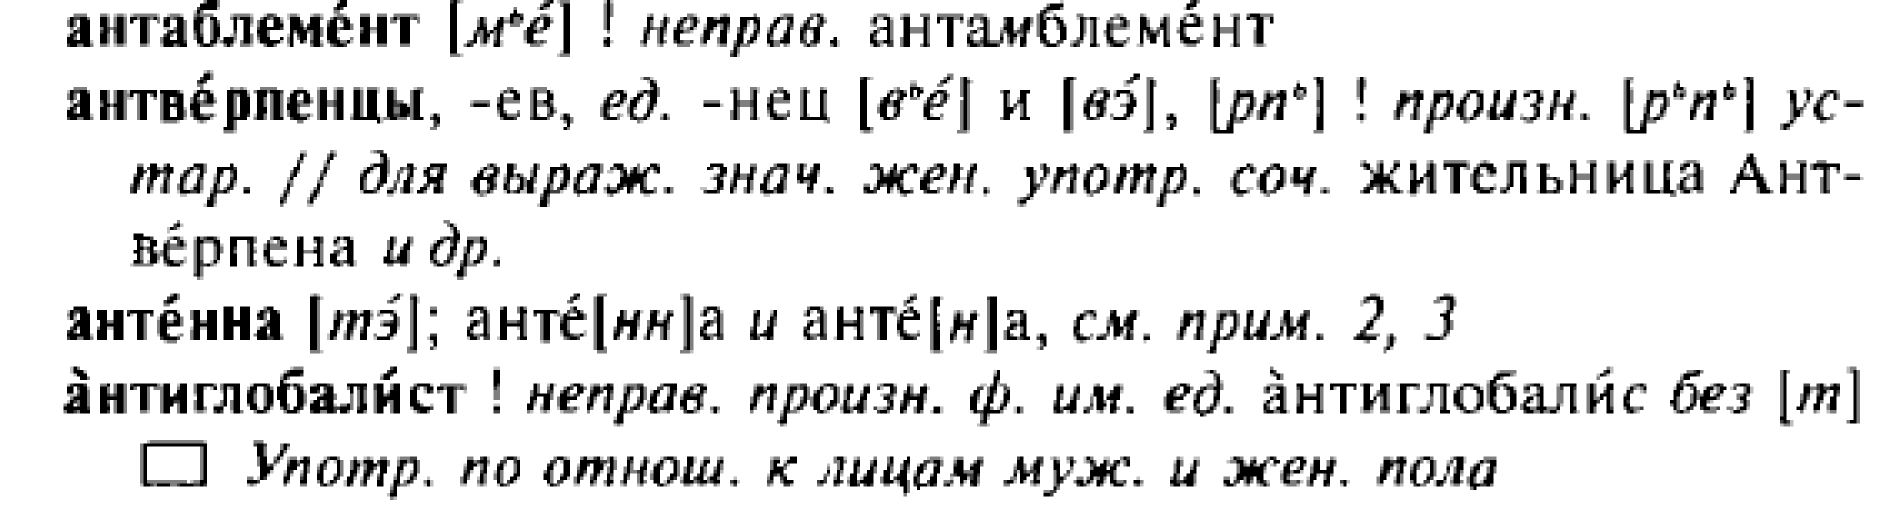
\includegraphics[width=\textwidth]{figures/orfo_example}
\end{minipage}
\begin{minipage}{0.3\textwidth}
\begingroup
\fontencoding{OT2}\fontfamily{wncyr}\fontsize{9pt}{12pt}\selectfont
\begin{Verbatim}
анестезиолог,ане->анэ | сте->стэ
анестезия,ане->анэ | сте->стэ
антенна,нте->нтэ
антисептика,исе->исэ
антитеза,ите->итэ
антитезис,ите->итэ
антитетический,ите->итэ
\end{Verbatim}
\endgroup
\end{minipage}
\caption{Links: Beispiel eines Eintrages aus \textcite[33]{rezni2005}. Rechts: Einige Formalisierungen für die Anwendung des Wörterbuches.}
\label{fig: orfo_example}
\end{figure}

Der Algorithmus von Itapov gibt keinen Hinweise auf den Umgang mit den velarisierten Konsonanten vor <e>, daher wird ein Wörterbuch verwendet, das aus den digitalen Fassungen von \textcite{rezni2005} und \textcite{kruk2008}\footnote{http://dazor.narod.ru/russkie/slovari/krukover/krukover-all.htm} zusammengesetzt wurde und die Änderungen für die Programmiersprache formalisiert wurden (Abbildung \ref{fig: orfo_example} rechts). Alle unbekannten Wörter werden der Graphie nach transkribiert. 

Bei der Palatalisationsassimilierung wird nach dem eingangs erwähnten Algorithmus vorgegangen, der dies nur zulässt bei /\textipa{s\super jt\super j}/, /\textipa{z\super jd\super j}/, /\textipa{n\super j\t{tS}\super j}/, /\textipa{n\super jt\super j}/, /\textipa{n\super js\super j}/, /\textipa{n\super jz\super j}/.

Doppelte Konsonanten bedeuten, dass sie lang ausgesprochen. Damit bilden sie für Silbentrennung zwei getrennte Konsonanten und werden dementsprechend getrennt oder nicht: Nach \textcite{vino1953} \textcyr{Анна} $\to$ \textcyr{Ан-на}, S5 $\to$ \textcyr{А-нна}. Um nach Itapov und co.\ zu entscheiden, ob die verdoppelten Grapheme auf phonetischer Ebene zwei Konsonanten bilden, gibt es einen Entscheidungsbaum, der Kriterien wie Betonung, Wortende oder -anfang oder, ob nachfolgendes Phonem ein Konsonant oder Vokal ist, einbezieht. Die eigene Implementierung wurde im Pseudocode-Beispiel in Algorithmus \ref{alg:cluster} dargestellt. Darin entscheidet zuerst die Position; sofern der Cluster in der Mitte des Wortes ist, gelten Regeln je nach Gruppe. Beispiele für Anwendung von ihm: \textcyr{балл $\to$ 1, русский $\to$ 1, суббота $\to$ 1, сумма $\to$ 2, аккорд $\to$ 1, рассада $\to$ 2}.

\begin{algorithm}
\caption{\textbf{Doppelter Konsonant (DK) -- Pseudocode-Lösung}}
\small
\label{alg:cluster}
\begin{algorithmic}
\If{DK am Wort\textsl{anfang}}
    \State Doppelter Konsonant
\ElsIf{DK am Wort\textsl{ende}}
	\State Ein Konsonant
\ElsIf{DK in Wort\textsl{mitte}}
    \If{Anderer Konsonant nach DK ($C_1C_1C_2$)}
        \State Ein Konsonant
    \ElsIf{DK besteht aus <\textcyr{б,в,ф,р,л,г}>}
    	\State Ein Konsonant
    \ElsIf{DK besteht aus <\textcyr{ж,т,д,з,с}>}
    	\State Zwei Konsonanten
    \ElsIf{Vokal vor DK betont \textbf{and} DK besteht aus <\textcyr{к,н,м,п}>}
    	\State Zwei Konsonanten
    \Else
    	\State Ein Konsonant	    
    \EndIf
\EndIf
\end{algorithmic}
\end{algorithm}
%\end{algorithm}
%TODO: write pseudo 
% Bei doppelten Konsonantengraphemen werden die Wörter ebenfalls in einem Wörterbuch nachgeschaut. Sofern das Wort aber nicht gefunden wurde, entscheidet die globale Häufigkeit nach der Abbildung \ref{fig: dou_con}, der eine eigene Auswertung des erwähnten Wörterbuches zu Grunde liegt. Wie man in \fref{fig: dou_con} sieht, nimmt die Konsonantenverbindung <\textcyr{нн}> den größten Anteil ein. Danach folgen die Paare <\textcyr{сс, лл, мм}>. Das Wörterbuch gibt für die Paare insgesamt drei Möglichkeiten zur Aussprache: als ein Konsonant, zwei oder erlaubt beide Varianten.
% Schwierig ist der letzte Fall, der in einer großen Zahl von Wörtern beide Varianten erlaubt. Hier muss der Algorithmus aber eine Entscheidung treffen: Es wird die Variante gewählt, die an sich die häufigste ist. Machine Learning Algorithmen wären die elegantere Wahl gewesen, aber da der gesammtelte Korpus für die meisten Konsonantenpaare zu klein ist\footnote{$N$ für bestimmte Paare: \textcyr{бб}: 8, \textcyr{гг}: 3, \textcyr{цц}: 4,\textcyr{вв}: 4. Median($Q_2$) allgemein: 31.}, kann und sollte man diesen Mechanismus nicht anwenden, da man sonst idiosynchratische Klassifikationen riskiert. Zusammengefasst: Im Fall, dass ein Wort nicht im internen Wörterbuch gefunden wird, lautet die Transkription für die Paare so:
% \begin{description}
% \item[Zwei Konsonanten] <\textcyr{сс, тт, цц, жж, вв, нн, дд}>
% \item[Ein Konsonant] <\textcyr{бб, гг, кк, лл, мм, пп, рр}>
% \end{description}
%TODO: machine learning vs manuell

% \begin{figure}[htbp]
% \centering
% 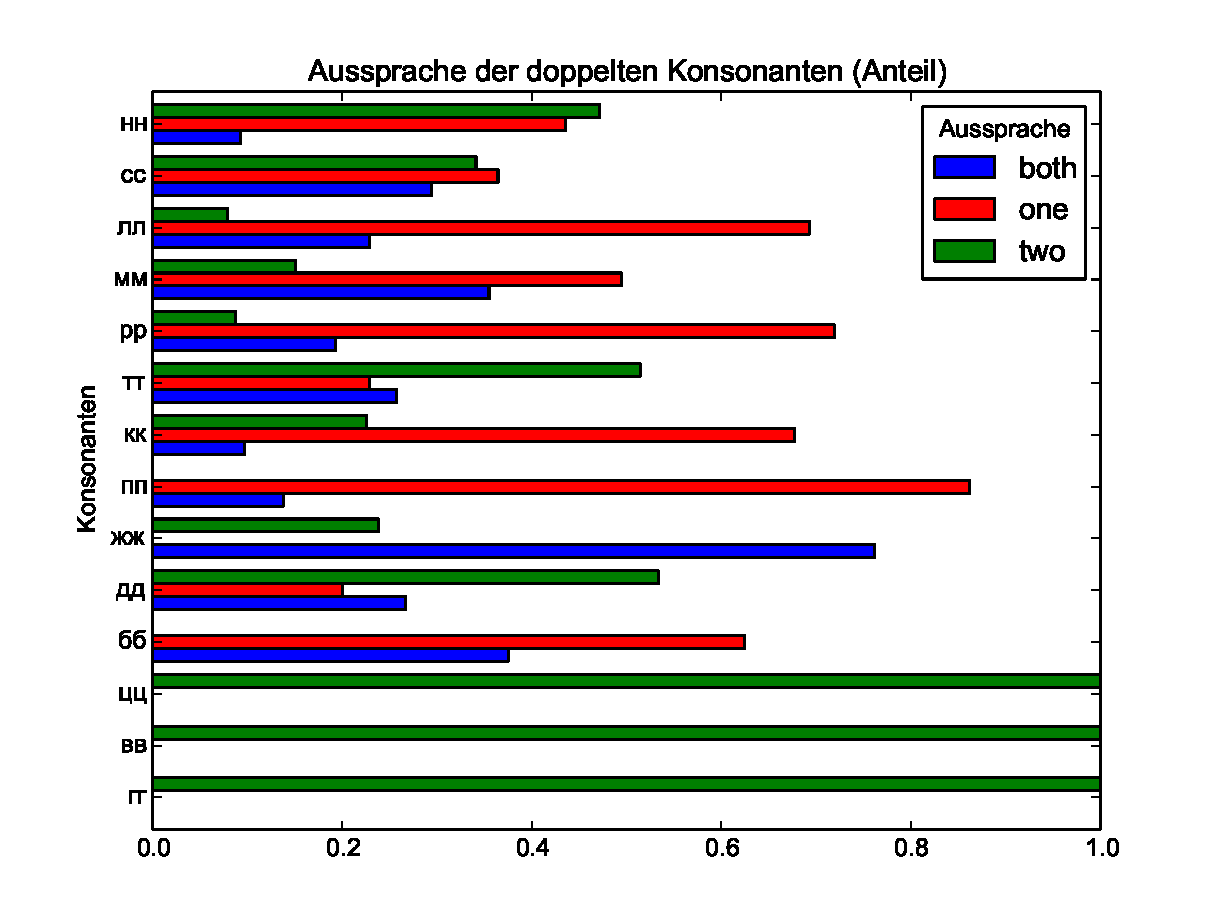
\includegraphics[width=\textwidth]{figures/double_cons_pd}
% \caption{Anteil der Aussprachevarianten von verdoppelten Konsonanten nach \textcite{rezni2005}. $N$=1383 -- $N$ = Anzahl der untersuchten Wörter}
% \label{fig: dou_con}
% \end{figure}

\subsection{Theoretische Grundlage zur Silbentrennung}
%TODO: read the oriinal jurafsky and cite the right page
Wie \textcite[406]{jurafsky2008} beschreiben, gibt es nicht nur mehrere Möglichkeiten wie man Silben segmentiert (unser \fref{sec:sylmodels}), sondern auch mehrere Arten, wie man dies automatisch tun könnte:
\begin{quotation}
One reason syllabification is a difficult computational task is that there is no completely
agreed-upon definition of syllable boundaries. Different on-line syllabified dictionaries
(such as the CMU and the CELEX lexicons) sometimes choose different syllabifications.
[\ldots]

Like much work in speech and language processing, syllabifiers can be based on
hand-written rules, or on machine learning from hand-labeled training sets.
\end{quotation}
Zumindest die erste Schwierigkeit umgeht diese Arbeit, indem es 5 Modelle implementiert und dem Forscher die Wahl überlässt.
Als Beispiel für Silbentrennung nennen sie die bereits erwähnten \textcite{goldwater2003}, die mit den Prinzipien Maximum Onset und SSP (Sonority Sequencing Principle) Regeln konstruieren, die über einzelne Sprachen hinweg verwendbar sind und mit diesem Ansatz eine sehr hohe Übereinstimmung mit sprachspezifischen Modellen erreichten.
Für Sprachen wie Italienisch, die dem SSP folgen, kann man in den neueren Ansätzen eine Genauigkeit von 100\% erreichen wie bei \textcite{iaco2011}.

\textcite[407]{jurafsky2008} stellen des Weiteren heraus, dass es drei Schritte zur Bestimmung einer Silbe gibt: "`Rule 1 forms nuclei at each syllabic segment, Rule 2a attaches onset consonants to the nucleus, and Rule 2b attaches coda consonants."'
Dies ist auch die Reihenfolge, die S1-5 machen. Es wird zuerst eine Silbe mit einem Nucleus gebildet, dann wird der gesamte Cluster provisorisch zu ihr hinzugefügt. Am Ende werden die Silben ausbalanciert, nämlich so viel vom Onset abgegeben bis er (und die Coda der vorherigen Silbe) der jeweiligen Regel entspricht.
Dies macht auch rein logisch Sinn: Wie \textcite[212]{bondarko1998}, ohne allerdings das Modell zu nennen, zeigt, hat das Russische 54\% offene CV Silben. Natürlich ist es nur ein Modell und die Zahlen können sich von Korpus zu Korpus ändern, doch die Tendenz zur einfachen und offenen Silbe spiegelt sich nicht nur durch die Intuition, sondern auch in diesen Zahlen wider.

Machine learning kommt für einen Silbenparser nicht in Frage, da es keinen großen (notwendig zumindest 1-2 Mio.), manuell getrennten Silbenkorpus fürs Russische gibt. Außerdem sind S1-3 eine Sammlung von manuellen Regeln und nicht statistischen. Als einzige (quasi) statistische Implementierung kann man nur die S4 betrachten, wenngleich es ein sehr simpler Mechanismus ist. Quasi und simpel deswegen, weil Kempgen keinen in Silben getrennten Text verwendet hat, sondern nur den konsonantischen Wortbeginn und das Wortende von Lemmata aus einem Wörterbuch.

%Im Übrigen fehlt für das Russische auch ein manuell annotierter Silbenkorpus, der machine-learning Algorithmen wie HMMs oder  Na\"{\i}ve Bayesian Classification ermöglichen könnte. Allerdings wäre selbst im Fall, dass ein manueller Silbenkorpus verfügbar wäre, die Frage nach dem Sinn berechtigt. Denn Annotierer müssten ja so oder so ein Modell aus Abschnitt \ref{sec:sylmodels} wählen oder eigene Regeln aufstellen. Diese Regeln könnte man dann noch besser als Algorithmus für den Computer schreiben wie im Fall der vorliegenden Arbeit anstatt sie manuell anzuwenden. Durch manuelle Annotierung eines Korpus gewinnt man also nichts.
%In phonetischen Korpora gilt dieser Gedanke ebenfalls. Auch da kann man zuerst in Phone segmentieren und dann durch Computerskripte alles zu Silben zusammensetzen.
%TODO: maybe cite harrison the phonetic
%Es ist allerdings sehr interessant, Daten von Probanden zu gewinnen wie bei \textcite{cote2011}, allerdings größeren Maßstabs. Psycholinguistische Daten wären als Perspektive zu betrachten, die machine-learning sinnvoll machen könnten.

\subsection{Programm-Mechanik}
%In diesem eher technisch Abschnitt soll die Code-Seite des Programms beleuchtet werden. Es würde sicherlich zu weit führen, alle internen Einzelheiten hier zu beschreiben. Eine Menge an Informationen lässt sich bereits aus den \textit{doc-types}(Dokumentation innerhalb des Codes) herauslesen. Da aber die technische Umsetzung weit von Vollendetheit entfernt ist, soll dem Leser ein größeres Bild vermittelt werden.

Der russische Text wird zuerst in pseudo-russische Wörter (\textcyr{лёхкий, серце}) übersetzt, da auch orthoepische Wörterbücher, auf denen das Programm teilweise basiert, so vorgehen. Danach wird das Wort in eine \textit{modifizierte} SAMPA-Kodierung (im Folgenden: Pysampa) übersetzt. Die Betonung auf Pysampa soll anzeigen, dass SAMPA, obwohl immer noch maschinenfreundlicher als die IPA, für NLP nicht perfekt ist. Intern, um bestimmte Stärken von der zu Grunde liegenden Code-Sprache zu nutzen, werden alle SAMPA-Zeichen, die aus zwei Graphemen bestehen (\textcyr{ч} $\to$ SAMPA: tS' $\to$ Pysampa: 4 oder \textcyr{ц} $\to$ SAMPA: ts $\to$ Pysampa: 3) zu unikalen Zeichen. Ansonsten wird bei der Iterierung der Eindruck erweckt, dass Affrikate oder palatalisierte Konsonanten aus zwei unabhängigen Zeichen bestehen. Durch Zusammenfassen zu einem Zeichen entgeht man diesem Problem. Alle Zeichen haben überdies die grundlegende Eigenschaft im ASCII-Zeichensatz zu sein und damit Probleme bei Konversionen zu umgehen.\footnote{Benutzung von ž oder č sind dadurch auch ausgeschlossen, da sie sich erst im erweiterten Zeichensatz cp1251 und UTF-8 befinden.} Die Umwandlung für Grapheme ist im Anhang \ref{sec:conv_graph} beschrieben.
%TODO: table with intern coding and SAMPA coding should be appended to the appendix

%TODO: write some more and make a picture 
Das Programm wurde stark für große Korpora optimiert, hauptsächlich durch einen \textit{dynamic programming} Algorithmus auf Grundlage von Sets.
Diese Optimierung lässt sich in Zahlen festhalten. Das Verarbeiten des 1MK dauert 480 Sekunden auf einem älteren Computer (Dual Core mit 2.4 GHz), der Testtext "`\textcyr{Интересно придумала}"' mit 179 Tokens braucht 1.4 Sekunden, pro Token wird der Unterschied klarer: 1MK--480 $\mu s$ (Mikrosekunden), der Testtext--7.8 $ms$ (Millisekunden): 1MK ist mehr als 16x schneller!

Mit den angesprochenen Verbesserungen lässt sich das Parsen des Korpus also um ein Vielfaches beschleunigen. Dies kann man in direkte Beziehung zu den Statistiken des Korpus in Verbindung bringen: Da die globale Set-Größe auch nur einen Bruchteil
%TODO: should be corrected: wrong set calc
der Tokens-Größe (124,000 vs. 1 Mio.) beträgt, muss man nicht jedes Wort direkt den Operationen des Programms unterziehen, sondern kann auf das Ergebnis von früheren Vorkommen zurückgreifen. Nehmen wir ein Wort \textcyr{дорогой}, das schon bereits einmal transkribiert und in Silben zerlegt wurde. Wenn es ein zweites Mal auftritt, ist es billiger (aus der CPU-Perspektive) das Wort aus einem "`Wörterbuch"' aller bisher berechneten Ergebnisse zu holen als das Wort neu zu berechnen. Das ist eine sehr einfache Implementierung von \textit{dynamic programming}.

% Sets sind eine mathematische-logische Richtung für sich. In vielen NLP Ansätzen sind Sets die Grundlage, nicht zuletzt ist ein unspezifischer Begriff wie Type bereits indirekt Ausdruck eines Set-Mechanismus. Denn in einem Set befinden sich alle einzigartigen Ausdrücke. Im Programmiersprachen bezeichnen Sets ebenfalls eine Datenrahmen mit einzigartigen \textit{items} plus einer Indexierung fürs schnelle \textit{retrieval}(Hervorholen aus dem Speicher). De facto sind im Punkt "`Types"' in Abschnitt \ref{sec:corpus_pars} alle Statistiken bloße Set-Analysen!
% %TODO: need better lit for set-logic *and* retrieval really the right good word?

% Zum Transliterieren und Parsen standen zwei Richtugen zur Auswahl: Ein Ansatz, der auf \textit{regular expressions} und einer auf \textit{low-level-string}-Funktionen beruht. Prinzipiell ist der erste sehr viel flexibler, weil er relativ vielfältige Verwendungen erlaubt. Der andere Ansatz hat eine klare (und begrenzte) Aufgabe, z.B. ersetzen von bestimmten Zeichen. Der Unterschied spiegelt sich praktisch darin wider, dass der letztere Ansatz 10-20x schneller ist.\footnote{Als Beispiel: http://stackoverflow.com/questions/5668947/python-string-replace-vs-re-sub} Als konkrete Anwendung kann man Pythons \textit{built-ins}(native, ohne Import benutzbare Funktionen) \texttt{replace} und \texttt{find} nennen, die wann immer möglich die externen Funktionen \texttt{re.sub} und \texttt{re.findall} ersetzten.
% % 
% Zur Rekursion muss man nicht viel sagen, außer dass auch sie Gegenstand zahlreicher NLP-Aufgaben ist\autocite{bird2009}. Obgleich Code-technisch recht teuer, ist sie eigentlich die intuitivste Implementierung der S4.
%TODO: Speed of code should be compared
%\bibliographystyle{unsrt}
\subsection{Die praktische Implementierung}
\label{sec:prac_imp}
Die praktische Implementierung geht nach einem Mehrebendesign wie der Parser fürs Italienische von \textcite{iaco2011} vor. Es gibt am Anfang eine Ebene, die den Text tokenisiert, d.h.\ in Wörter trennt. Innerhalb des vorliegenden Korpus wurde dies bereits gemacht, normalerweise läuft dies auf Grundlage von Leerzeichen.

Danach wird jedes Wort auf einen Eintrag in einem zu Grunde liegenden Wörterbuch geprüft, ob phonetische Operationen nötig sind wie in \fref{sec:phon_alg} aufgezählt. 
%Dies wird durch Lemmata geleistet; auch dann ist der Algorithmus kompliziert, denn man muss die phonetische Operation auf das Token übertragen. Die Formalisierung wurde in \fref{fig: orfo_example} vorgestellt. 
Die phonetischen Änderungen führen zu einer pseudo-phonetischen Form.

\begin{figure}[htbp]
\centering 
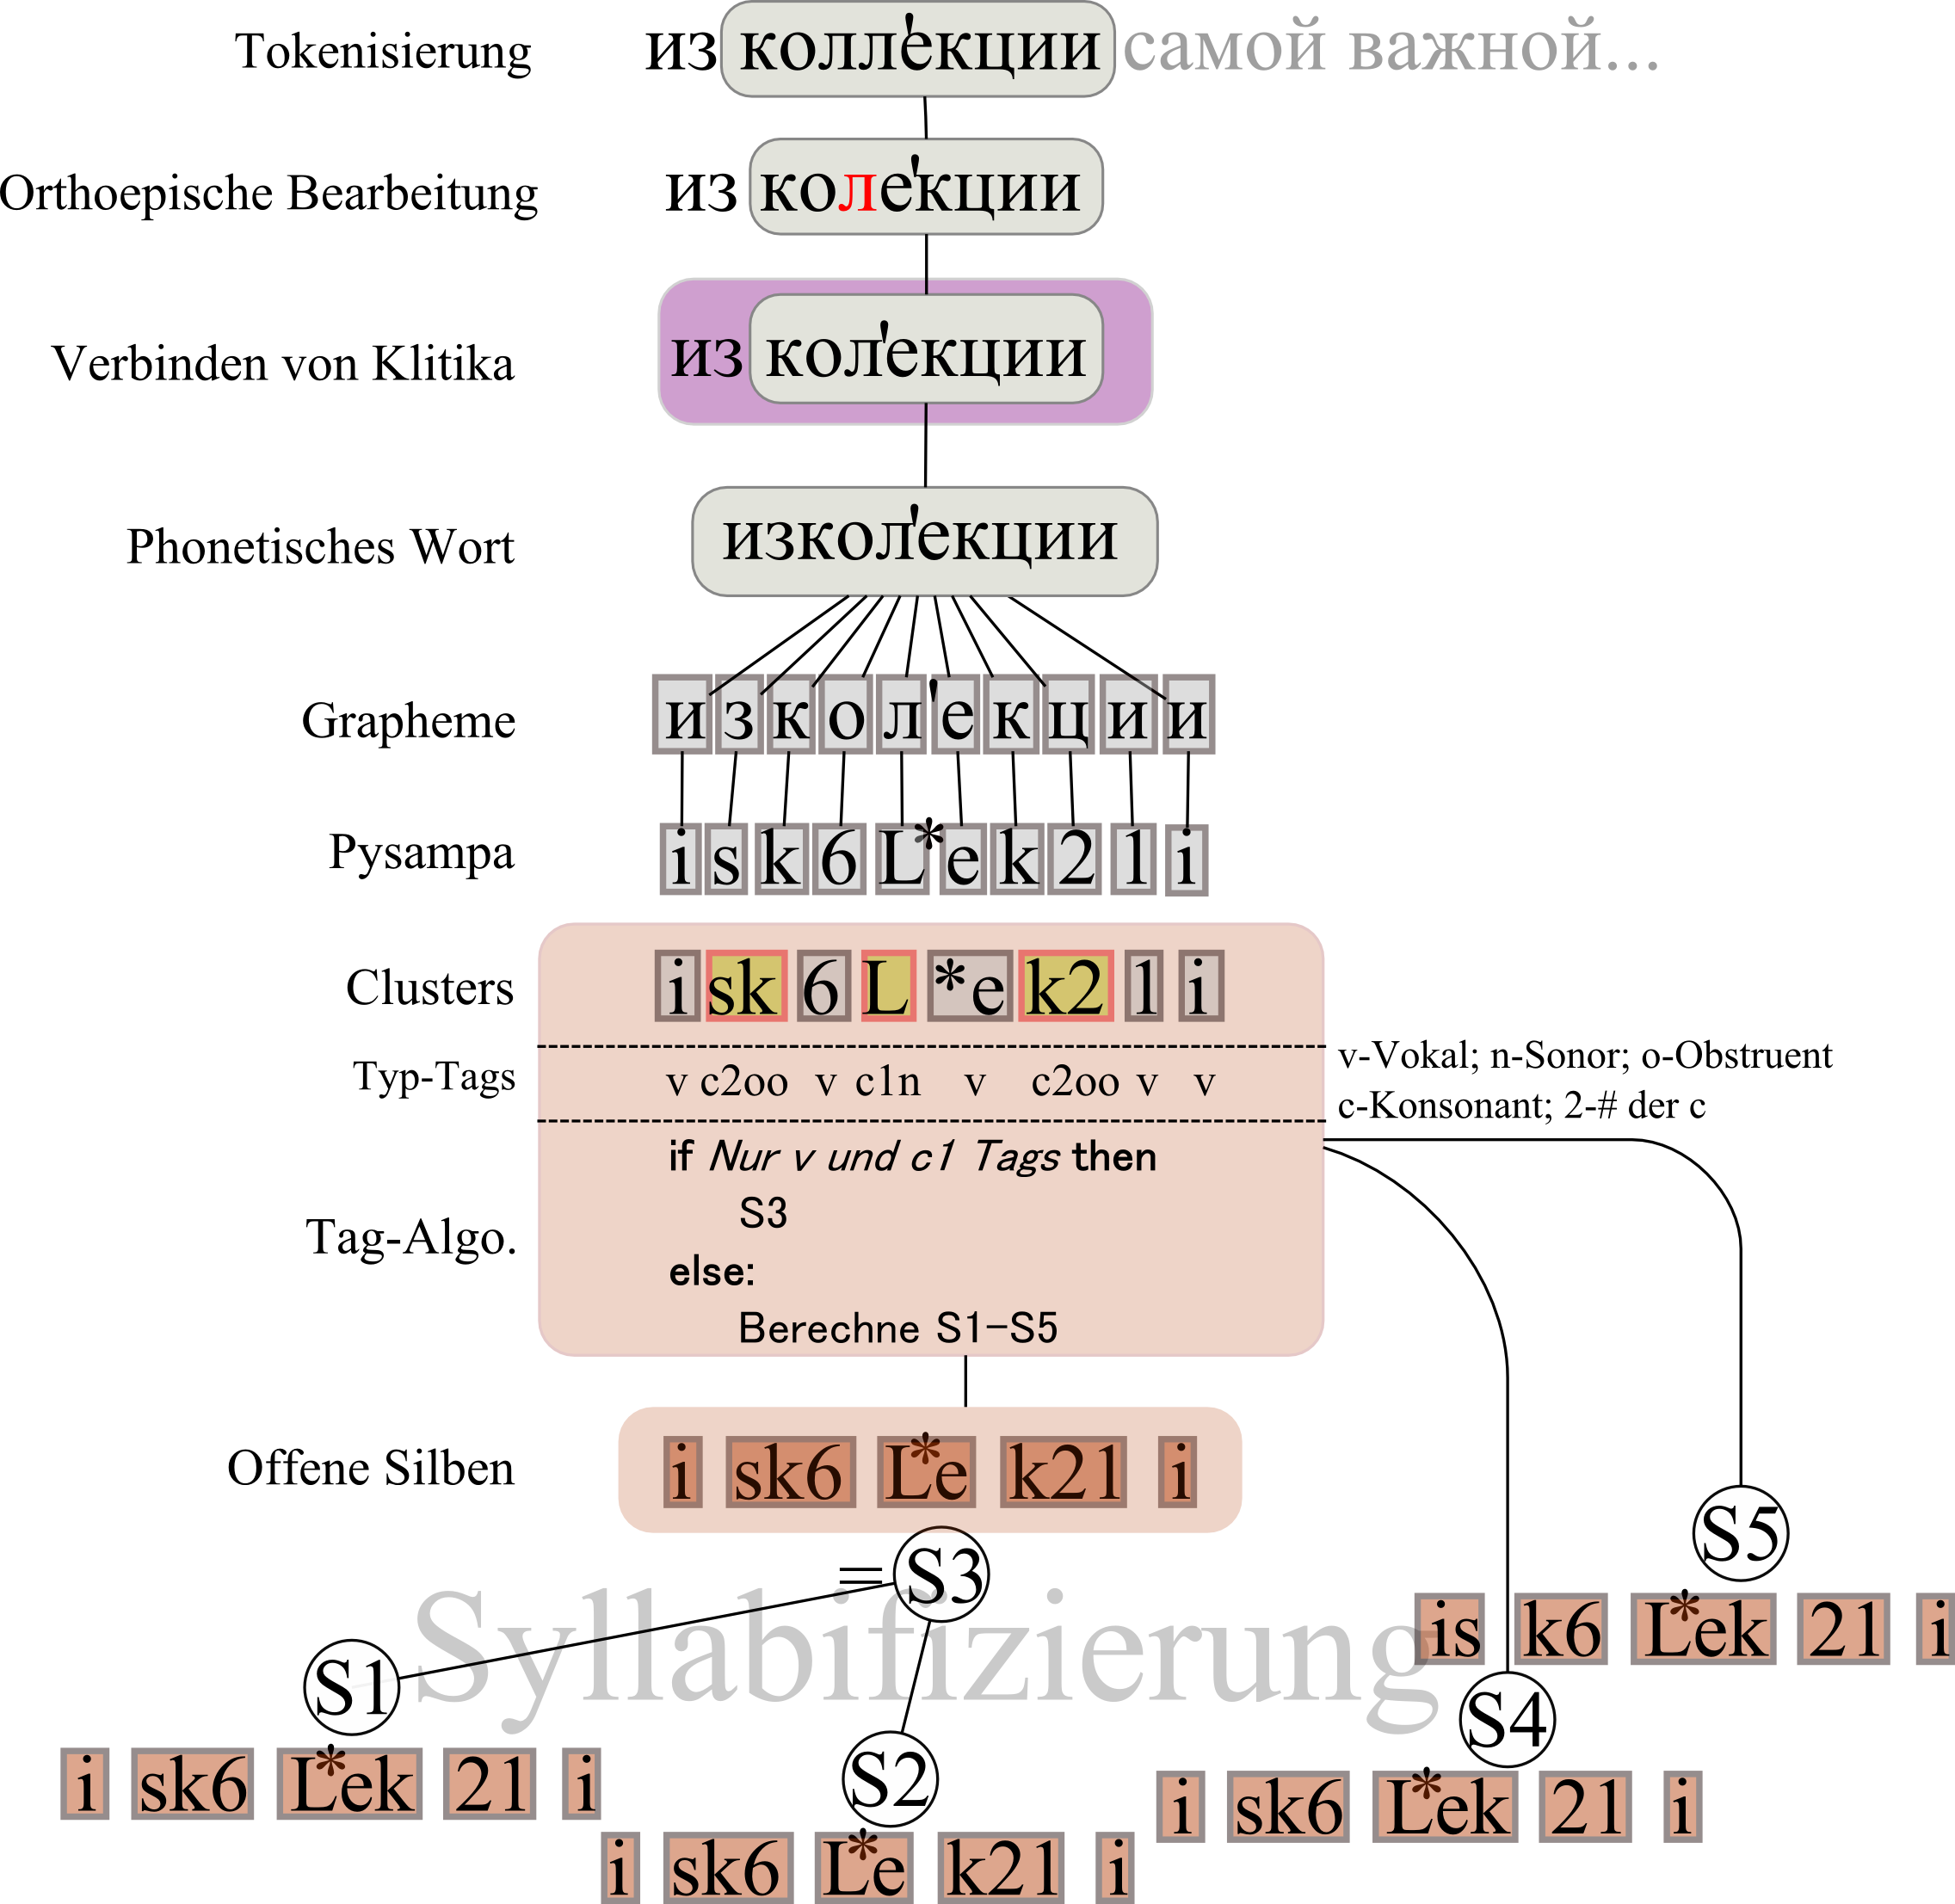
\includegraphics[width=0.8\textwidth]{figures/syllaru_system.png}
\caption{Bildliche Darstellung des Silbentrennungsprogramms.}
\label{fig: syl_sys}
\end{figure}

Als nächstes werden die Klitika mit dem Hauptwort verbunden, sodass ein phonetisches Wort entsteht -- dies ebenfalls zunächst auf der graphemischen Ebene. Diese Operation wird auf den ganzen Text angewendet. 
Auf Grund der Erfahrung aus dem 1MK werden auf dieser Ebene nach dem Verbinden der Klitika alle Verbindungen aus der Analyse getilgt, die nicht-kyrillische Zeichen enthalten, keine Betonung haben (aber mehrere Vokale) oder Abkürzungen sind. Im 1MK wurden auf diese Art 30,000 Wörter der ersten Art eliminiert, 60.000 der zweiten Art und 2400 Wörter der dritten Kategorie plus einer unbestimmten Zahl von Klitika, die diese Wörter umgeben haben. Nach diesem Filter blieben nur noch 784,000 phonetische Wörter (Tokens) für die Analyse, die sich aus 124,000 Types zusammensetzen bzw.\ 117,000 für den später gewählten Subkorpus.
Danach werden die einzelnen Grapheme in Pysampa transkribiert. 

Der nächste Schritt ist es, die Allophone in konsonantische und vokalische Intervalle zu teilen. 
An dieser Stelle passiert auch ein Tagging der Cluster, um zu bestimmen, ob ein Wort vielleicht nur aus einfachen (V)CV-Verbindungen (c1(x) und v Tags) besteht und daher das S3 ausreicht. Dies spart bei ca. 42\% der Wörtern unnötige CPU-Zyklen (=Diese Wörter haben eine \textit{Set size} von 1).
Im Falle, dass die Tags Hinweise auf Cluster geben (z.B. c2oo oder c2on usw.), werden die Silbenmodelle ausgerechnet. S1 und S2 werden auf Grundlage von S3 bzw.\ der Ebene der offenen Silbe bestimmt.

S4 und S5 wurden zuerst auch von dort aus berechnet. Nach einigen Tests aber erwies sich eine Abzweigung von der Clusterebene direkt zu den Modellen effektiver, da, wie man später sehen wird, bei diesen Modellen weniger offene Silben herauskommen. 

%Die Analyseschritte gehören nicht mehr zum Programm, sondern werden durch externe Bibliotheken in R, pandas und SQL gemacht. Die sehr simplifizierte Darstellung in Abbildung \ref{fig: syl_sys} gibt die technische Seite nur unzureichend wider. Im Anhang%
%make appedix with figures of code execution
%finden sich komplettere Graphiken, die verdeutlichen, dass technisch zwei Klassen zum Transkribieren und Syllabifizieren arbeiten, sowie ein \textsl{Memoizer}, der Wiederholungen von Rechenoperationen verhütet. 
% Die Klassen teilen sich nach \textsl{object-oriented-programming} in mehrere Funktionen und so weiter bis ein harter Kern aus C-Funktionen erreicht ist -- danach übernimmt die CPU die Arbeit.
\newpage

\section{Statistische Auswertung des Korpus}
\label{sec: stat_tst}

%Auf Grund der im letzten Kapitel beschriebenen Schwierigkeiten eine 1:1 Übersetzung von Graphemen zu Phonen zu leisten, werden die Statistiken eher quantitativ und rudimentär ausfallen. Ob nun aber ein Graphem e die Weichheit anzeigt oder nicht, ist für das Silbenskelett ohne Bedeutung sowie auch für die Offenheit der Silbe oder die Anzahl der Silben im Wort. Problematisch ist es für das S4, da Kempgen zwischen palatalisiert und nicht-palatalisiert unterscheidet. Allerdings finden sich in seiner Arbeit keine Anhaltspunkte, wie er mit den Schwierigkeiten der Orthoepie umgegangen ist. Möglicherweise hat er die graphemische Oberfläche ohne eine Kontrolle durch Orthoepie benutzt.
 
Wie die Analyse des Korpus in \fref{sec:corp_stats} gezeigt hat, gibt es zwei große Teile. Da das Ziel dieser Arbeit ein Vergleich der Silbenmodelle ist, beschränkt sich die Analyse auf den standard-Korpus. Die zusätzliche Variable des Subkorpus ist eine etwas schwierige Frage, da der eine Subkorpus 3x größer ist. Wie \textcite{baayen2001} gezeigt hat, hängt die Wörtervielfalt von der Größe des Textes oder Korpus ab. Da Silben Wörter bilden, würde für Silben das Gleiche gelten. Für einen Vergleich müsste man nach Monte Carlo-Methoden aus den beiden Subkorpora ein zufälliges, gleich großes Sample ziehen -- damit würde aber sich der Schwerpunkt dieser Arbeit auf den Vergleich der Subkorpora  verschieben.

\subsection{Globale Statistiken}
Im gewählten standard-Subkorpus bekommt man nach dem Parsen von ca. 600,000 Wörtern 1,688 Mio. Silben, was 2.8 Silben pro Wort ausmacht. Da die Silbenanzahl bei allen Modellen gleich ist\footnote{Bei S4 und S5 wurde 1 einzige (!) Silbe weniger gefunden, was wohl ein Kodierungsfehler im Text ist.} (vereinfacht: Silbenanzahl entspricht immer der Anzahl der Vokale), erlaubt dies die Verteilungen der Silbenanzahl anzuschauen ohne die Modelle einzubeziehen. Die Statistik hilft dabei, zu entscheiden, auf welcher Ebene die folgenden Statistiken ausgeführt werden sollen: Types oder Tokens.
 
\begin{figure}[htbp]
\centering
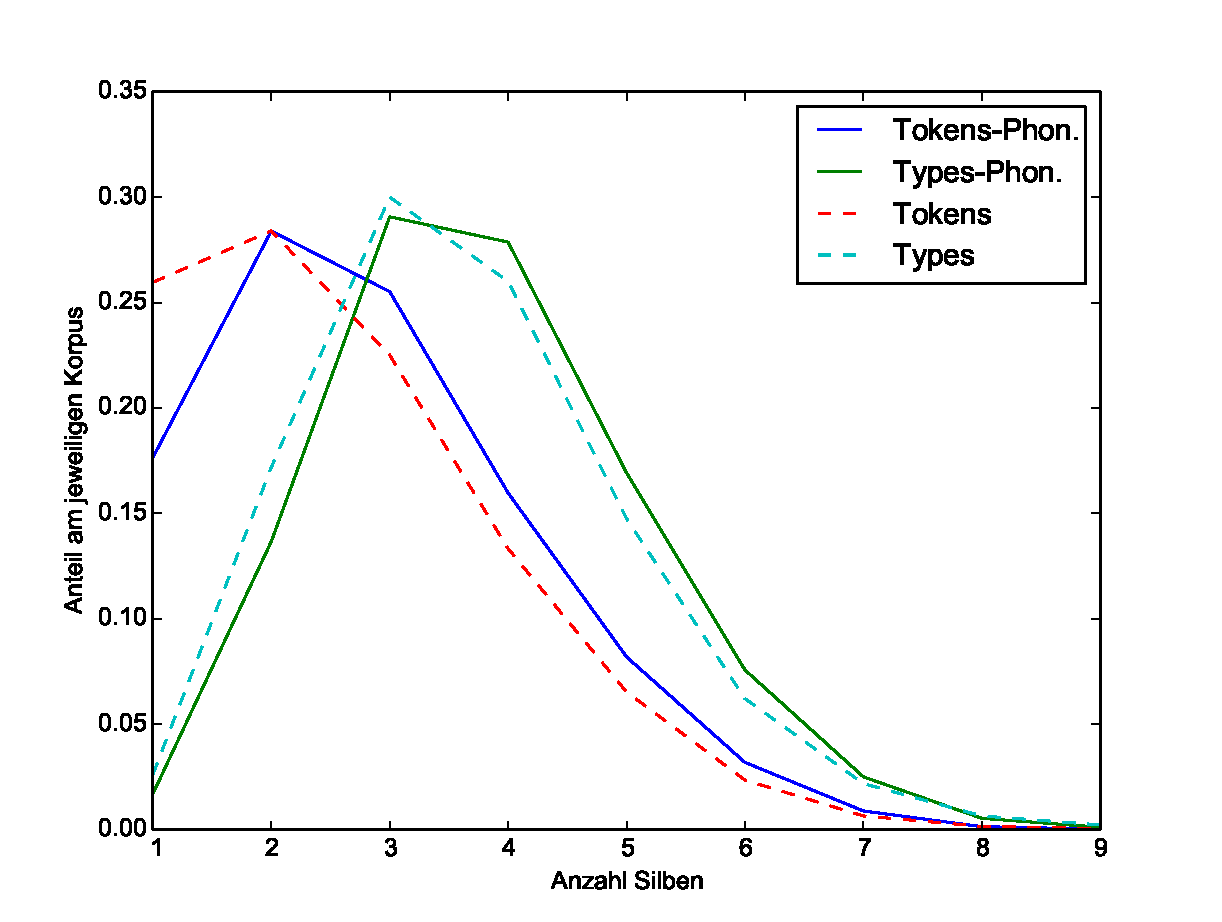
\includegraphics[width=0.8\textwidth]{figures/syls_stats_glob.pdf}
\caption{Silbenverteilungen auf den Ebenen der Types und Tokens (gestrichelt), dazu nach dem Verbinden der Klitika (durchgehend, mit "`Phon."'-endend).}
\label{fig: syl_glob}
\end{figure}

Man kann in \fref{fig: syl_glob} sehen, dass die Tokens-Verteilung viel stärker nach links verzerrt ist, während die Types-Verteilung eher symmetrisch aussieht. Dies lässt sich mit dem Bezug zur Wortstatistiken erklären, denn einfache (1 oder 2-silbige) Verbindungen wie \textcyr{я, ты, и} machen auch den größten Teil des Russischen National-Korpus bei den Häufigkeiten aus, sowie tendenziell auch jeder anderen Sprache. Was in der jeweiligen Ebene interessanter ist, ist der Effekt von verbundenen Klitika. Bei Tokens kann man eindeutig sehen, dass viele einsilbige Wörter (sprich: viele Klitika) innerhalb von größeren Wörtern aufgegangen sind und damit die Unterscheidung in längeren Wörtern verursachen. Bei Types ist die Unterscheidung ebenfalls mit dem Wirken der Klitika zu erklären. Auch wenn natürlich hochfrequente Wörter wie Klitika keine Rolle auf Typesebene spielen, so haben sie doch durch Verbinden auf der Tokensebene zu einem phonetischen Wort für mehr Vielfalt (sprich: mehr Types) \textit{und} längere Wörter gesorgt.\footnote{Vereinfacht: In einer Liste [a,b,a,b,c,b,d,d,c] mit b als Klitika haben wir 9 Tokens und 4 Types (Durch.-Länge: 1). Durch Verbinden von b mit jeweils folgendem Item bekommen wir 6 Types (Durch.-Länge: 1.5). Dies ist der Unterschied zwischen Types und Types-Phon.}

Nun muss aber eine Entscheidung im Sinne der Analyse getroffen werden: \textit{Eine} Entscheidung wurde schon beim Design des Programms getroffen, nämlich Silben innerhalb von phonetischen Wörtern zu untersuchen. Die obige Hinzunahme von Korpora ohne Verbindung mit Klitika sollte nur den Effekt der Maßnahme verdeutlichen.
Bei der wichtigen Entscheidung zwischen Tokens (Tokens-Phon.\ in \fref{fig: syl_glob}) und Types (Types-Phon.) wählt man wegen der besseren Verteilung und Abwesenheit von Frequenzeffekten von Klitika die Types-Ebene.

\subsection{Vergleich der Silbenmodelle}
Um eine Vergleichsform zu finden, lässt sich am besten zuerst zusammenfassen, was das Programm für Daten über einen Text ausgibt. 
\begin{enumerate}
  \item Silbenstatistiken und ihre Frequenz wie in \fref{tab: 10high_std} links.
  \item Wörter und ihre Segmentierung zwischen den Modellen + Anzahl der unterschiedlichen Segmentierungen wie in \fref{tab: 10high_std} rechts. Ssi ist dabei eine Abkürzung für Set size -- wie groß also der Set (einzigartige Segmentierungen) für ein Wort ist.
\end{enumerate}

Die Wahl des zweiten Weges würde bedeuten, dass der Schwerpunkt sich auf die Eigenschaften der Wörter verlagern würde wie die Anzahl ihrer Laute, Frequenz, Google Ngram-Profil usw. Schaut man sich die Häufigkeiten der einzelnen Ssi's an, sieht man aber, dass von den 117,000 Types fast 42\% keinen Unterschied zwischen den Modellen ergeben haben (=Ssi von 1; Ssi von 5 bedeutet, dass es 5 verschiede Trennungen gab). Eine gepaarte Pearson-Korrelation ergibt daher für alle Modelle einen hohen Wert zwischen 0.98-0.99, nach Spearman immerhin nur 0.93-0.98. Dieses Zwischenergebnis zeigt, dass die Modelle allesamt ähnliche Silbenfrequenzen ergeben.
 
 \begin{table}[htbp]
 \caption{Links: Ein kleiner Teil (5 von 16,878) an Silben mit Frequenzen und ob sie ausgewählt wurden (An(alyse)?). Rechts: Häufigkeiten der Set size (Ssi) und ihr Anteil am Types-Subkorpus sowie Beispiele. "`*"'--Betonung; links und rechts ohne Beziehung.}
 \label{tab: 10high_std}
\small
 \begin{tabular}{r|ccccccc}
 \toprule
$\sigma$ &     s1 &     s2 &     s3 &     s4 &     s5&An? \\
 \midrule
*ent   &   2    &2    &2    &2    &2 &$\times$\\
*i        &5   &93  &117  &104   &27& $\checkmark$\\
2*e      &70  &154  &215  &118  &169 &$\checkmark$\\
*us      &28  &0  &0  &0   &21& $\times$\\
*al       &8    &8    &2    &7    &8& $\checkmark$\\
 \bottomrule
 \end{tabular}
\quad
\begin{tabular}{c|ccl}
\toprule
Ssi&$N_{Ssi}$&Anteil&Beispiel\\
\midrule
1&49,676 &42.3\%& \textcyr{декабр*я}\\
2&50,177&42.7\%&\textcyr{б*ублики}\\
3&14,002&11.9\%& \textcyr{моск*овской}\\
4& 3079&2.6\%&\textcyr{напросп*екте}\\
5&328&0.2\% &\textcyr{инсп*ектора}\\
\bottomrule
\end{tabular}
 \end{table} 


Dieses Ergebnis ist aber vom statistischen Standpunkt nicht zufriedenstellend, schließlich wollen wir wissen, \textit{wie} sich die Modelle unterscheiden. Dafür reicht eine solche Korrelation nicht aus und vor allem die Daten benötigen eine weitere logische Spezifizierung. Zum einen wählen wir im Folgenden für den Vergleich nur die Wörter, die auch Unterschiede gezeigt haben (Ssi>1) und wir setzen eine weitere Filterung ein, um Ausreißer zu filtern. Dies ist dringend notwendig, da nach der Einbeziehung des Kriteriums Ssi>1 noch immer die Daten sehr ungleichmäßig sind. Der Median der Summe aller Modelle ist 52, der Mittelwert 465. Die untere Quartile beträgt 16, verteilt auf 5 Modelle ergibt das $\leq$ 3.2 Silben an durchschnittlichen Beobachtungen für die unteren 25\% der Silben. Auch dieses Zwischenergebnis erbringt die Erkenntnis, dass auf Silbenebene ähnliche Gesetze gelten wie auf Wortebene. Eine geringe Zahl von Silben nimmt den größten Teil der Vorkommen ein. In Zahlen ausgedrückt: 50\% der Vorkommen werden von nur 42 Silben eingenommen. Extremer würde es sicher sein, falls wir noch die Frequenzeffekte einbezogen hätten (Tokens-Ebene). 

Das Problem ist in der Textanalyse nicht neu und wurde schon im obigen Unterkapitel angesprochen. Als erster Schritt wurden zuerst alle Zeilen aussortiert, die auch nur einen einzigen Wert 0 hatten. Die Lösung für die weitere Analyse ist, um \textcite{lebart1998} zu folgen, zunächst einen \textit{threshold} (eine Untergrenze zur Berücksichtigung von Beobachtungen) anzusetzen. Dazu gibt es keinen bestimmten Wert; wichtig ist, eine aussagekräftige Datengrundlage für weitere Analysen zu erhalten. Wir wählen zunächst einen Wert von 25, pro Modell also durchschnittlich 5 Beobachtungen, was eine Voraussetzung für den $\chi^2$-Test ist. Bezogen auf Tabelle \ref{tab: 10high_std} heißt dies, dass man alle Zeilen aussortiert, die in der Summe weniger als 25 erbringen. 
Die \fref{fig: freq_map} zeigt die bisher erfolgte Filterung in chronologischer Abfolge von der Tokensebene zu Types und dann zu Silben bis zum uns interessierenden Teil der Silben. Die besprochene Filterung \textit{innerhalb} des Silbensets kann man auch anhand von Beispielen in \fref{tab: 10high_std} links (Spalte "`An?"') nachverfolgen, wobei Häckchen die Zugehörigkeit zur schließlichen Auswahl anzeigt. 
 
\begin{figure}[htbp]
\centering  
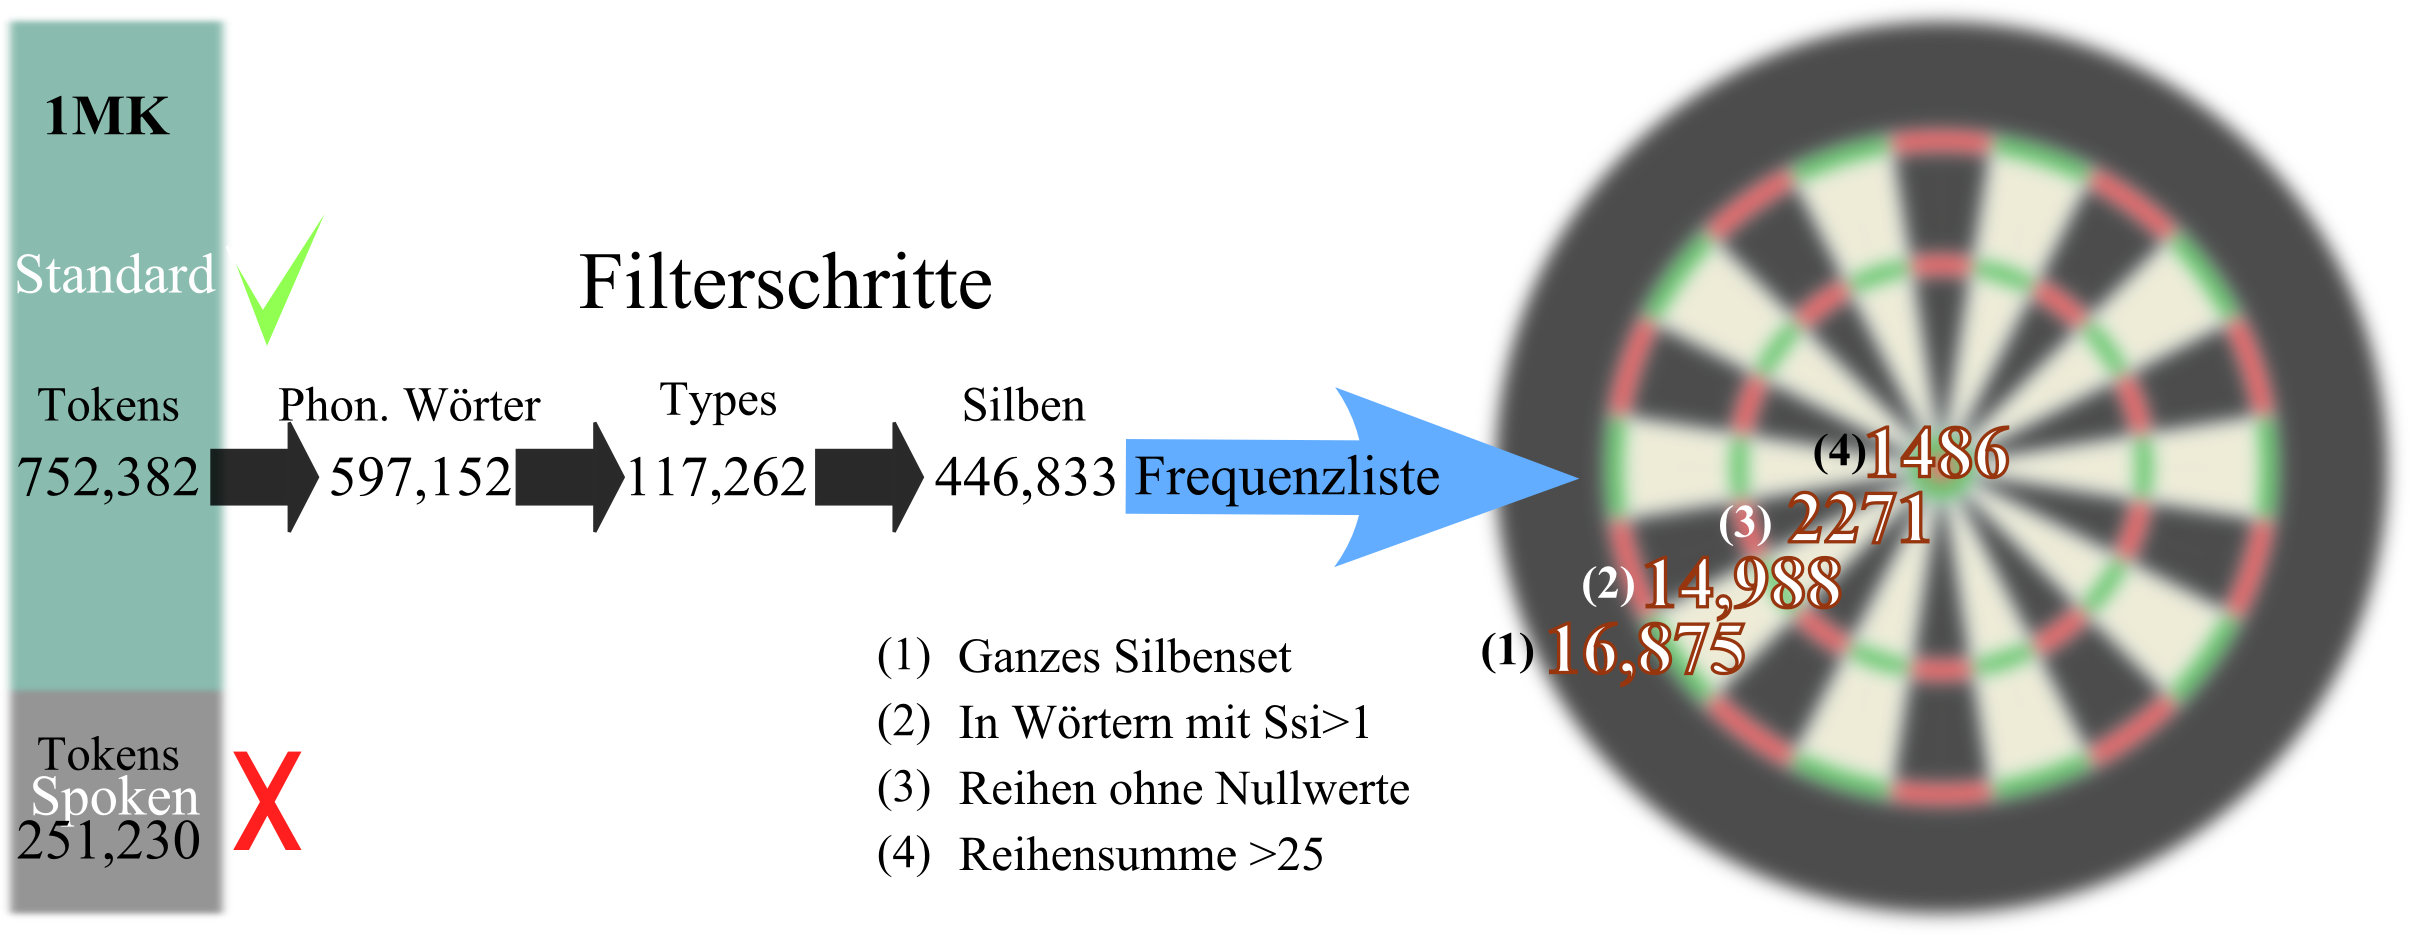
\includegraphics[width=0.95\textwidth]{figures/freq_map2.png}
\caption{Die unterschiedlichen Schritte der Filterung; jeder Schritt nach rechts übernimmt die Bedingung ($\sigma \ni \ldots$) des linken Schritts. Silben in der Mitte der Frequenzliste haben die größte Aussagekraft.}
\label{fig: freq_map}
\end{figure} 

\subsection{Correspondence Analysis}
Ein $\chi^2$-Test ist -- dem großen Sample wegen -- wenig überraschend hochsigfikant (p>0.01). Die verbleibenden 1486 Silben von ehemals über 16,000 dienten folglich für eine Correspondence Analysis, die von \textcite{baayen2008} und \textcite{lebart1998} angewandt wurde für \textit{count data}; eine Schwestertechnik für Messdaten ist die principle components analysis (PCA). PCA und CA behandeln (vereinfacht gesagt) die Daten wie einen multi-dimensionalen Raum, in dem durch Einsetzen von Ebenen versucht wird, möglichst viele Datenpunkte zu treffen. Je nachdem wie erfolgreich eine Ebene ist, vereint sie mehr oder weniger Erklärungspotenzial, das in \textit{eigenvalues} gemessen wird bzw.\ im Plot als Anteil an der gesamten Standardabweichung. Nach \textcite[141]{baayen2008} hat die CA aber einen weiteren praktischen Vorzug: "`The attractiveness of correspondence analysis resides in the possibilities it offers for visualization"'. 

Alle 1486 Silben in ihrer graphischen Form einzubeziehen, würde die gleiche Anzahl an Kategorien bedeuten (der Silbenpool ist ja ein Set).
Deswegen soll abstrahiert werden: 
Es sollen die in den vorherigen  Abschnitten benutzten Begriffe wie Onset, Coda benutzt werden. Zum Beispiel soll eine Silbe "`sP*ek"' (aus \textcyr{напросп*екте}) charakterisiert werden als mit Obstruent beginnend (Plot 1) und endend (P2), 1 Konsonant in Coda (P3), 2 Konsonanten im Onset (P4). 
 
\begin{figure}[htbp]
\centering
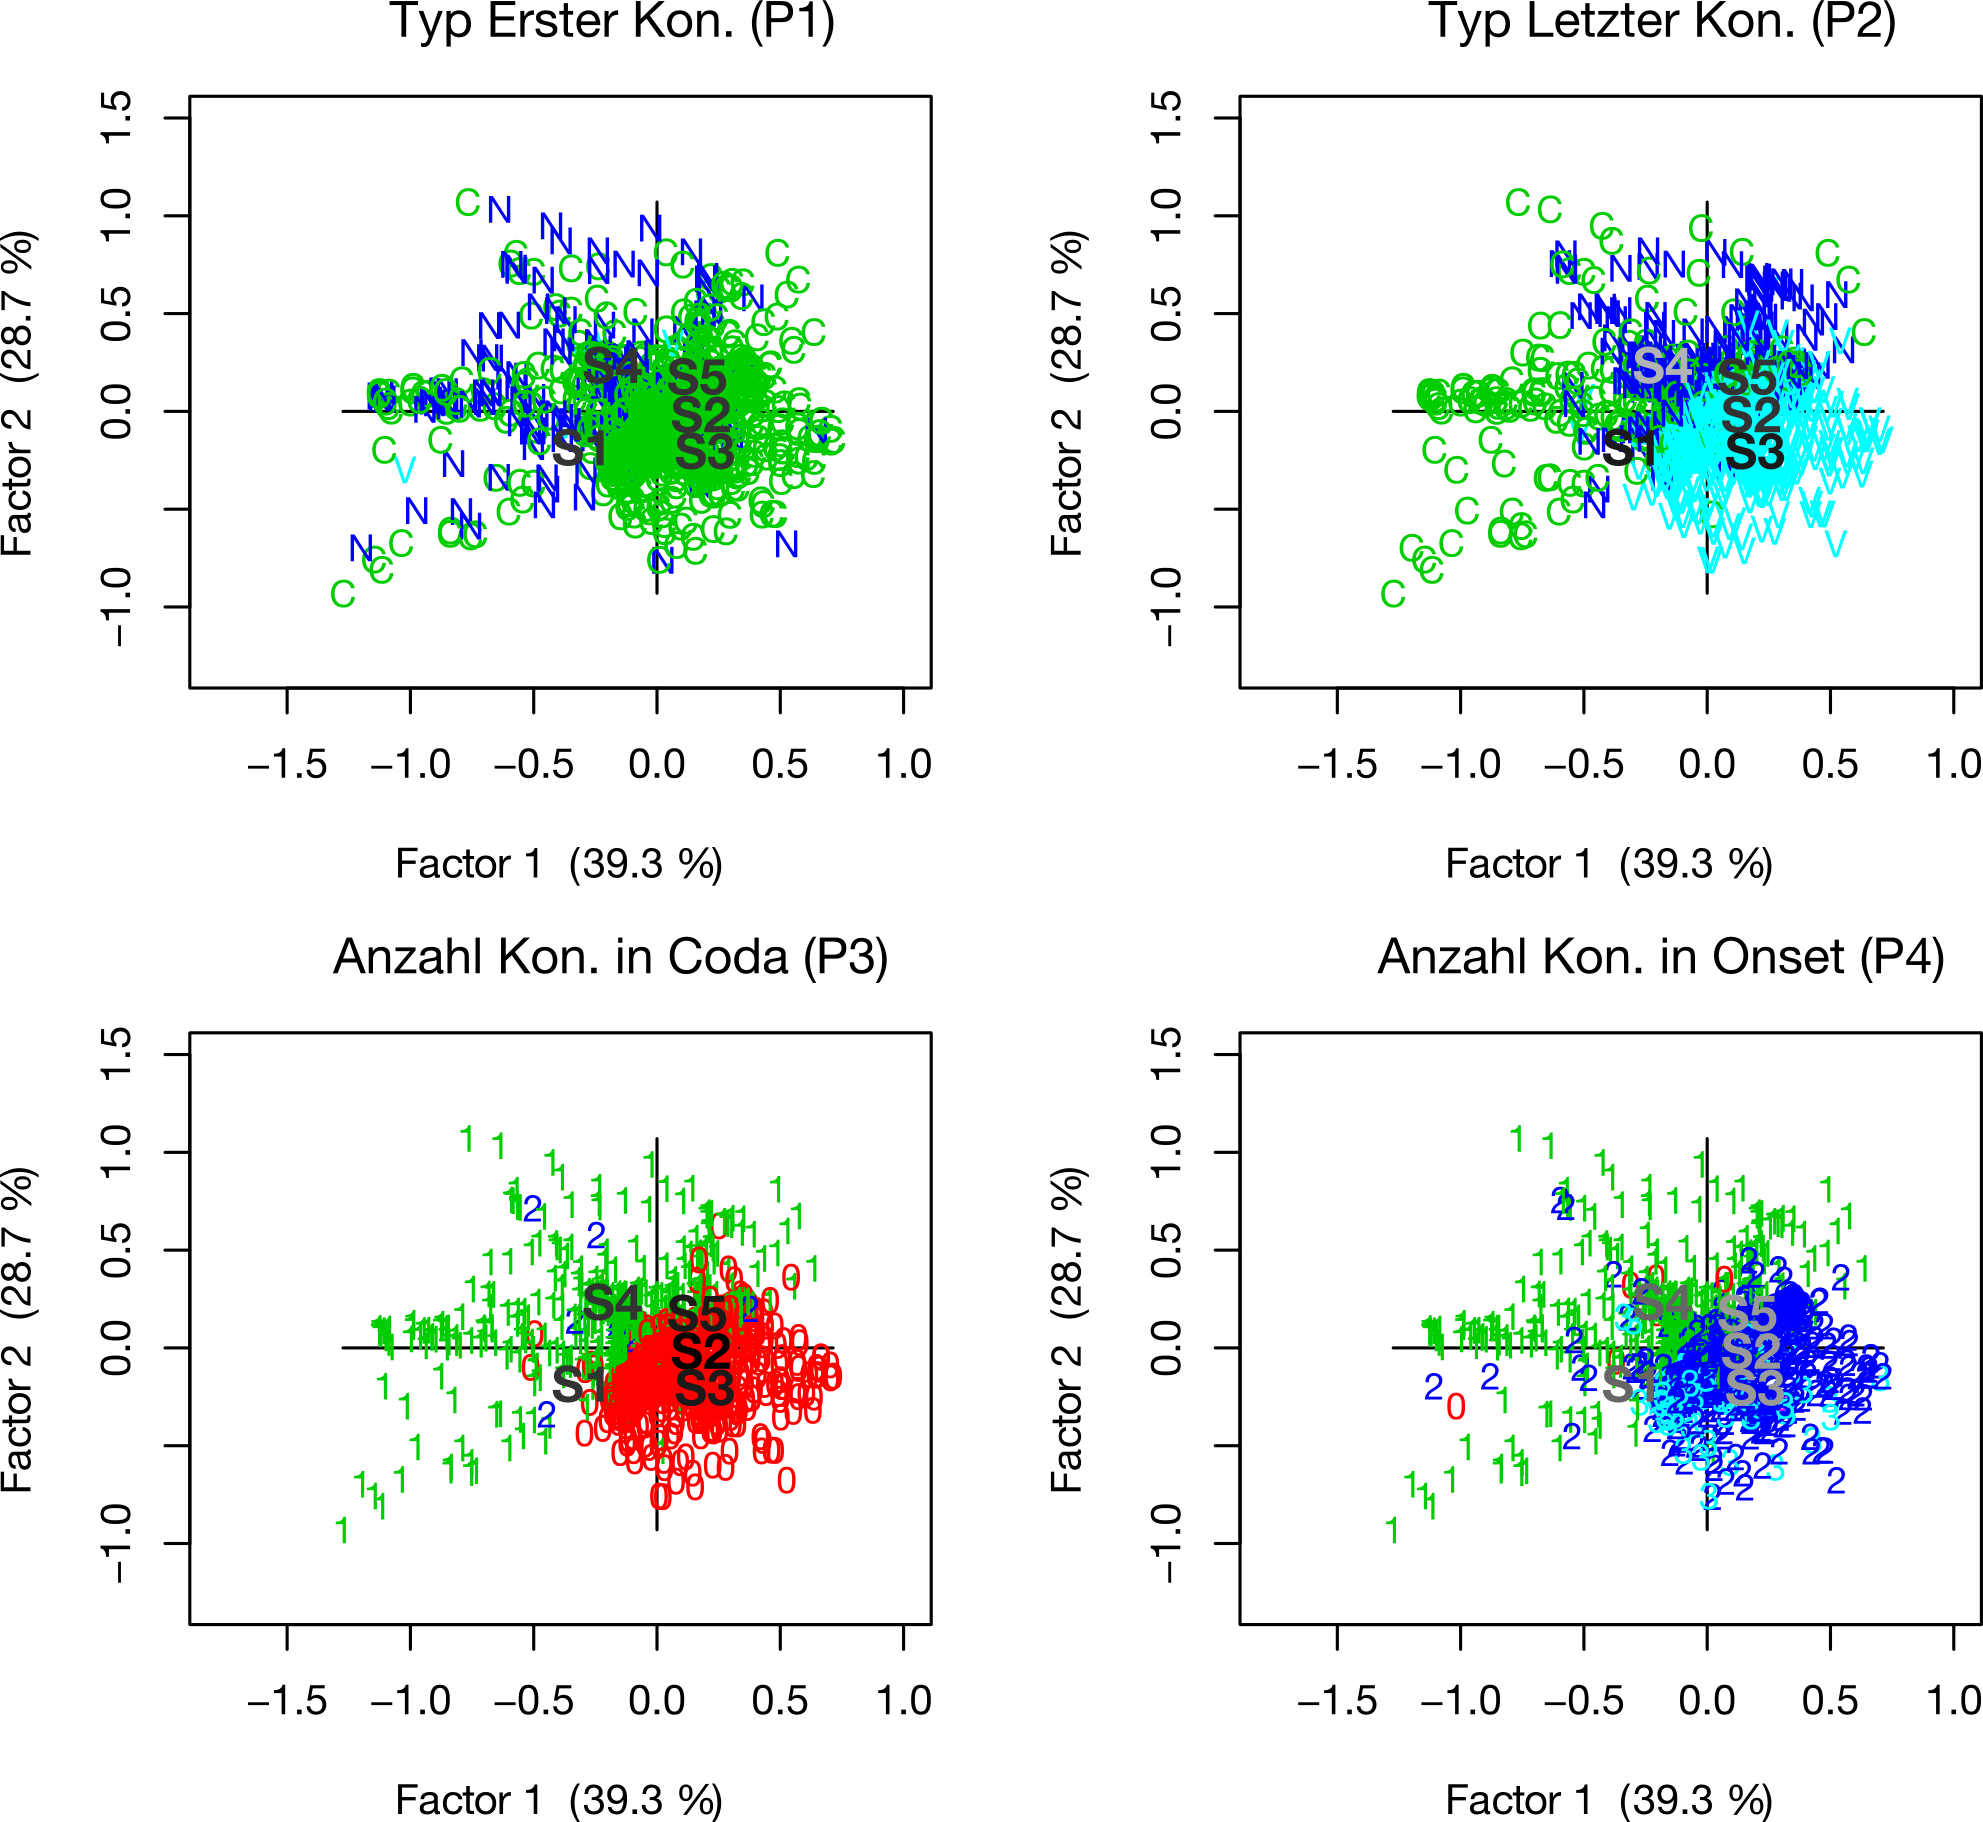
\includegraphics[width=0.75\textwidth]{figures/ca_syls.png}
\caption{CA der Silbenmodelle. Statt graphischer Form der Silben sind ihre Eigenschaften gezeigt. Kon.--Konsonant. Farben von S1-5 wurden jeweils wegen der Sichtbarkeit angepasst.}
\label{fig: ca_syls}
\end{figure} 

Zunächst wurde mittels der umgewandelten Frequenzen in Ränge eine CA-Faktor-Matrix erstellt mit 4 Faktoren, wobei die ersten beiden (X1 und X2) am meisten die Varianz zusammenfassen und daher im folgenden für die Analyse verwendet werden.
Danach wurden die vorgestellten vier Silbenkategorien nacheinander in \fref{fig: ca_syls} eingebracht worden. Der erste Plot (P1) scheint auch gleich die Clusteeffekte teilweise aufzulösen. Die diagonale Grenze, die durch fast alle Plots geht, erklärt sich aber vor allem durch den zweiten Plot. Er zeigt, dass das Bondarko-Modell tatsächlich ein Extrem markiert und zwar durch die Eigenschaft, dass der letzte Laut in der Silbe ein Vokal ist. Ebenfalls befindet sich S2 innerhalb der vokalischen Silbenendung. S5 und S1 befinden sich am Übergang zur Gruppe mit konsonantischer Silbenendung. Andererseits befindet sich S4 abseits der anderen Modelle in einem deutlichen Cluster konsonantischer Endungen -- hier wiederum zwischen Sonoren und Obstruenten. P3 und P4 imitieren die Aussage von P1 und P2 mit anderen Eigenschaften: Die Gruppen trennen sich durch die Eigenschaft, wie viel die Modelle im Coda oder Onset erlauben. S3, S2 erlauben eindeutig mehr Konsonanten im Onset, was zu Lasten der Codas geht, bei S4 ist andersherum. S5 und S1 liegen auf der Grenze. 

Bei der Interpretation sagt P2 (Silbenauslaut) am meisten aus; er erklärt die Tendenz von S1 nach links, von S5 nach oben und S4 zwischen S1 und S5. Im Bereich von S5 und S2 liegen deutlich mehr Silben mit Sonoren am Ende. Wir wissen aus der Theorie: Für S2 ist die Anwesenheit eines Sonors im Cluster entscheidend, um ihn zur Coda zu zählen. S5 zählt Sonore ebenfalls zur Coda, sofern nach ihm ein Obstruent kommt. S1 kann auch Obstruenten in die Coda nehmen, sofern die Betonung auf der Silbe ist. Dieser Fall spiegelt sich durch die Verortung innerhalb der Obstruenten-Coda wider. S4 hat dagegen ein Coda-Profil, dass sich zwischen S5 und S1 orientiert.

Die Korrelationen in \fref{tab: cor_mat} mit den einzelnen Faktoren sind für den ersten Faktor (X1) unbedeutend; nicht nur der visuelle Eindruck bestätigt, dass der 2. Faktor entscheidend ist, sondern auch die hohen Korrelationen mit den jeweiligen Silbeneigenschaften. Dass so gut wie alle Korrelationen ($\geq$ 0.1) signifikant sind (p>0.05), soll angesichts des großen Samples von 1486 Silben nicht überraschen. X1 wird wohl größtenteils entweder eine andere latente Eigenschaft widerspiegeln oder einfach eine zusammengefasste Variation sein. An der negativen Korrelation zwischen Anzahl der Konsonanten in Coda und im Onset sieht man, dass eine \textit{inverse} Beziehung existiert; die beiden Silbeneigenschaften haben des Weiteren eine hohe Korrelation mit X2 -- dem Faktor, der für die Clustering-Effekte auf der vertikalen Achse verantwortlich ist. Ergänzend dazu ist vor allem die Eigenschaft des letzten Lautes in der Silbe mit der Anzahl der Größe des Onsets und Coda stark korreliert (0.6, -0.72), sodass die Variation, die X2 ausdrückt, vor allem durch die Silbeneigenschaften entsteht und die Silbenmodelle unterscheidet.

Zusammengefasst bestätigt sich der Eindruck, dass die Coda den Unterschied in den Silbenmodellen ausmacht. Dies drückt aber eine größere, \textit{latente} Eigenschaft aus, nämlich die Offenheit bzw. Geschlossenheit. S4 bevorzugt eindeutig eine geschlossene Silbe, während S1 und S5 eine gemischte Tendenz aufweisen allerdings mit anderen Vorzeichen (Obstruent vs. Sonor). S3 -- das zeigt sich nicht nur in der Theorie, sondern auch in Statistiken -- präferiert eine offene Silbe.

\begin{table}
\centering
\caption{Spearman-Korrelationsmatrix der CA-Faktoren mit Silbeneigenschaften. Namen oben sind abgekürzt.}
\label{tab: cor_mat}
\begin{tabular}{r|rrrrrrr}
\toprule
{} &         X1 &         X2 &   LL&  EL&      KC&     KO\\
\midrule
X1        &       1.00 &  &&&&\\
X2        &      -0.12 &       1.00 &      &&&\\
Let. Laut&       0.01 &      -0.69 &       1.00 &       &&\\
Ers. Laut&       0.18 &      -0.30 &       0.23 &       1.00 &       &\\
Anzahl Kon. in Coda    &       0.07 &      -0.72 &       0.96 &       0.26 &       1.00 &      \\
Anzahl Kon. in Onset&       0.02 &       0.60 &      -0.53 &      -0.26 &      -0.55 &       1.00 \\
\bottomrule
\end{tabular}
\end{table}
\newpage

\section*{Abschließende Worte und Ausblick}
\addcontentsline{toc}{section}{Abschließende Worte und Ausblick}

Im Rahmen dieser Arbeit wurde mehrere Dinge praktisch angegangen und gelöst. Es wurden einige grundlegende Begriffe (Silbe, NLP) zum Rahmen der Arbeit definiert.

Danach wurden konkrete Silbentheorien und die Hauptgemeinsamkeiten und -unterschiede dargestellt. Dabei wurden russische und westliche Ansätze zunächst theoretisch gegenübergestellt. 

Die Korpusbeschreibung stellte die Weichen für eine weitere Eingrenzung der Daten. Anschließend wurde die technische Umsetzung vorgestellt. Dabei wurden Schwierigkeiten festgestellt, die nicht optimal in dieser Arbeit gelöst werden konnten (Transkription); allerdings konnten für die meisten Probleme formale und systematische Ansätze aus der Russistik angewendet werden. Es wurde unter Einbeziehung der aktuellen Theorien eine grundsätzliche Entscheidung zu Gunsten von manuellen Regeln gefällt, die auch den Charakter der Daten widerspiegeln.

Die wirkende Mechanik konnte zunächst auf einem technischen und abstrakten Niveau  (Kap. "`Programm-Mechanik"') vorgestellt werden und dann auf einem praktischen ("`Die praktische Implementierung"'). Es zeigte sich, dass ein Programm durch ein modulares Design am besten für Texte geeignet ist und bei Korpora Geschwindigkeit und Effizienz am besten sicherstellt.

Der statistische Abschnitt rekapitulierte einige Korpusparameter und brachte dies mit Schwierigkeiten der Analyse in Verbindung. Ein Ergebnis war, dass im Russischen unter Hinzunahme von Frequenzeffekten kaum Unterschiede zwischen den Silbenmodellen existieren. An den Zahlen zeigte sich außerdem das, was man von der Silbe als Brücke zwischen Wort und Phonem erwarten würde: 117,000 Types lösten sich in 16,000 Silben auf, die sich wiederum aus 44 Phonemen bzw. Allophonen zusammensetzten.

Andererseits zeigten sich ähnliche Frequenzeffekte wie auf Wortebene, dass nämlich eine geringe Anzahl von Types einen großen Teil an Beobachtungen einnahm. 
Daher wurden im Weiteren die Daten nach bestimmten Kriterien gefiltert bis ein aussagekräftiges Sample erreicht war. An diesem konnten Unterschiede durch Anwendung der CA und Einbeziehung von ouverten und latenten Silbeneigenschaften  aufgezeigt werden, die eine gewisse Clusterung nach Eigenschaften verursachten. Diese Clusterung konnte man gut mit den theoretischen Eigenschaften erklären.
\\

Die Ergebnisse sind interessant, reizen aber das Potential der Daten und des Programms nicht komplett aus: Die Wortebene wurde nur für die Filterung von Ssi's verwendet sowie zum Gewinnen der Silbenfrequenzen, man kann aber von Wörtern ausgehend schauen, inwiefern  ihre Eigenschaften mit Ssi oder ihre Trennung mit ihrer Herkunft (Wörter aus romanischen Sprachen nach SSP?) korrelieren. In Bezug auf Silben könnte man die Korpusgrundlage vergleichen z.B. mit Spoken-Teil oder Lehrbücher, wo Betonungen gesetzt sind, mit den Subkorpora. Dafür müsste man allerdings ein Modell wählen, denn sonst hätte man neben Silben und Korporatypen als Variablen auch Silbenmodelle. Die vorliegende Arbeit entschied sich durch Filterung dafür, den Korpus als Kontrollvariable zu nehmen. Die weitere Perspektive könnte der Versuch eines Klassifikators von Texten sein, der auf Grundlage von Silben das Genre eines Textes bestimmt.

Es wurde viel Zeit investiert in eine einfache, aber auch flexible Struktur, die als Basis für weitere Ergänzungen dienen kann und soll. Die weitere Entwicklung soll ermöglichen, dass man einfache psycholinguistische Daten erheben kann und diese mit der Datenbank abgleichen kann, als Fragestellung würde sich anbieten: Welchem Modell ist die Segmentierung einer Person ähnlich? Andererseits müsste man in Zukunft einige andere Richtungen bearbeiten: Automatisches Betonungssetzen, Zusammensetzen von Phonsegmentierung in Praat-Textgrids zu Silben, Erweiterung der phonetischen Wörterbuchbasis, um eine Transkription mehr von Daten und weniger von formalen Regeln abhängig zu machen. Außerdem könnte man eine graphische Oberfläche für das Programm schaffen.
\newpage

\addcontentsline{toc}{section}{Literatur}
% \bibliography
\printbibliography
%\addcontentsline{toc}{section}{Literatur}
\newpage

\appendix

\section{Technische Spezifikationen}
\label{sec:tech_spec}
%\subsection{Codegrundlagen}
Die Statistiken wurden mit Hilfe der Code-Sprachen R und Python sowie indirekt mit C gemacht. Bei R\footnote{http://www.r-project.org/} wird die aktuelle Version 3.0.1 verwendet, Python\footnote{http://www.python.org/} und die Statistikbibliothek \textsl{pandas} \autocite{mckinney2012} werden in der Standardimplementierung in C (CPython, nicht zu verwechseln mit Cython) verwendet. Die benutzte Version ist 2.7.4, das getestete Betriebssystem ist Windows XP, das Programm 
%TODO: Unter Win8,Vista testen
wurde aber ebenfalls auf Windows 8 und 7 erfolgreich getestet. Unter Mac oder Unix OS steht eine lauffähige Version (noch) aus, die unkompilierten Skripte mit der Endung \texttt{.py} sollten auf jeden System laufen, wenn man Python 2.7 installiert. Die kompilierte Fassung auf dem USB-Stick ist auf Windows zugeschnitten. Vorrangig ist es als Skript für den Python Interpreter gedacht; auf dem Stick befindet sich eine allein lauffähige \textit{cmd}\footnote{Windows Command Line}-Anwendung. Das neueste Skript wird auf der github-Plattform zu finden sein, wo die Entwicklung nach der vorliegenden Arbeit weiterverlaufen wird.

Für Python wird neben pandas (10.1) auch lxml\footnote{http://lxml.de/} benötigt. 

Zur Command Line Anwendung: Mit dem Programm werden 5 Texte geliefert. 3 belletristische Texte und zwei zufällige Texte aus dem 1MK. Ihre Metadaten kann man lesen, wenn man es in einem Editor oder besser in einem beliebigen Browser (Firefox, IE usw.) öffnet. 

Zum Starten muss man auf \texttt{syl\_parse.exe} klicken. Dann parst das Programm automatisch den Ordner "`test\_data/mk1"' mit seinem gesamten Inhalt. Dies ist nützlich, wenn man sich von der ruscorpora-Stiftung eine eigene Kopie des 1MK besorgt. Die gesamten Files legt man in den Ordner und lässt sie Parsen. Silbenstatistiken zum 1MK sind übrigens auch so mitgeliefert im Ordner "`syl\_data"', nur nicht die Ausgangstexte oder die Wörter.

Wenn man allerdings etwas anderes als den 1MK parsen will, so sollte man im Auge behalten, dass das Programm zuallererst auf das Format des Korpus abgestimmt wurde. Alle anderen Texte außer den Testtexten können Probleme verursachen (Betonungszeichen müssen immer mit "`'"' markiert sein, Satzzeichen usw.).
Will man Testtexte außer dem 1MK parsen, so muss man in die Command Line von Windows gehen und dann z.B. folgenden eintippen (Zeilen mit "`\#" -Kommentar):
\begin{verbatim}
#wechselt zum Ordner mit der .exe
E:
cd E:/comp_syl_parser
syl_parser test_data/lit_texts txt
#Programm startet und gibt die Etappen aus: read done, map done usw.
\end{verbatim}
Alternativ dazu kann man auch die Datei \texttt{syl\_parser.bat} anklicken. Sie startet automatisch das Parsen der Belletristik-Texte.

Die geparsten Files sowie die Silbenstatistiken finden sich dann im Ordner "`outp\_data"'.
\newpage

\section{USB-Inhalt}
Es wurde sich für ein USB-Stick als Datenträger entschieden, weil das Programm auch einen Speicherplatz braucht, um die Parser-Ergebnisse zu schreiben. CD's oder DVD's sind aber nur durch einen Brenner beschreibbar und nicht durch ein kleines Programm. Sehr wichtig ist folgendes: Alle Dateien sind in cp1251 Enkodierung und nicht UTF-8, um also Daten mit Nicht-ASCII Zeichen in Excel oder sonst wo zu bearbeiten, sollte man als Decoder cp1251 wählen, sonst würde man nur seltsame Zeichen lesen.

Es sind 4 Ordner vorhanden:
\begin{description}
\item[comp\_syl\_parser] Hier befindet sich eine kompilierte .exe Anwendung für den Parser. Um diese zu benutzen braucht man nichts zu installieren, sondern es reicht nur auf \texttt{syl\_parser.exe} zu klicken. Dann wird automatisch ein Teil des 1MK geparst. Für die anderen Testtexte sollte man wie zuletzt im Anhang \ref{sec:tech_spec} beschrieben vorgehen, d.h. zum Beispiel die \texttt{syl\_parser.bat} Datei anklicken. Alles andere in diesem Ordner ist irrelevant. Es sind einfach Bibliotheken, die für das Programm notwendig sind. 
\item[uncomp\_syl\_parser] Hier ist eine unkompilierte Fassung sämtlicher Funktionen zu finden. Man kann alle Files mit der Endung .py in jedem beliebigen Editor öffnen und lesen. Das File \texttt{syl\_parser.py} ist das, was man als Python-Anwendung startet. Man muss dafür aber die Dependenzen pandas und lxml installieren. Alle anderen Files übernehmen verschiedene Funktionen wie orthoepisches Anpassen (\texttt{orfo\_prep.py}), Verbinden der Klitika (\texttt{parse\_txt\_prep.py}) und Transkription (\texttt{new\_syl\_class.py}).
\begin{itemize}
  \item Der Ordner \textbf{orfo\_data} beinhaltet das orthoepische Wörterbuch mit ca. 900 Wörtern und die Tabellen von Kempgen im .csv Format. Alle Dateien werden von dem Programm benötigt, daher sollte hier nichts entfernt werden oder modifiziert werden. Öffnen und lesen geht aber ohne Probleme, solange man die Kodierung nicht verändert.
  \item Der Ordner \textbf{test\_data} beinhaltet alle Files zum Parsen, so den 1MK im Ordner mk1 und die Belletristik Texte in lit\_texts. mk1-Ordner enthält zwei zufällig ausgewählte Files. lit\_texts-Ordner enthält eine Geschichte von M. Zošenko "`Interesno pridumala"' sowie den Text "`Tolstyj i Tonkij"' von A. Čechov und "`Bargamot und Garyska"' von L. Andreev. Die letzten zwei Texte wurden aus Wikipedia heruntergeladen und für die Verarbeitung durch das Programm modifiziert.\footnote{http://ru.wikisource.org/wiki/\textcyr{Категория:Тексты\_с\_ударениями}} Der erste Text wurde für ein anderes Projekt bereits in einigen Worten modifiziert, es wurden aber Betonungen ergänzt.
  \item In den Ordner \textbf{outp\_data} werden die Daten geschrieben, die man geparst hat: Ein File mit Wörtern und den 5 Segmentierungen und dazu Silbenstatistiken basierend darauf.
 
\end{itemize}
\item[syl\_data] Hier sind einige Silbenstatistiken aus dem 1MK (\texttt{syl\_share\_spokstan.csv}) zu finden, getrennt nach Spoken- und Standard-Subkorpora, allerdings wurden sie vor einer kleinen Korrektur des Programms gemacht, sodass sie 23 Silben weniger haben als eigentlich da ist. Dazu gibt es Statistiken zum ganzen Korpus (\texttt{syl\_compcorp.csv}), die auch aktuell sind, allerdings wurde dazu keine Unterscheidung zwischen Spoken und Standard gemacht. Dazu wird die CA (\texttt{factor\_postca.csv}) mit den Faktoren und den Eigenschaften sowie den Ausgangswerten (\texttt{syl\_preca.csv}) geliefert. Wörterdaten kann man durch die Lizenz nicht zugänglich machen. Sofern man aber den Korpus bekommen hat, kann man ihn durch Ablegen der .xhtml-Files in den Ordner "`/test\_data/mk1"' parsen lassen. Dazu startet man einfach die \texttt{syl\_parser.exe}. Dann sollte der Output geliefert werden.
\item[thesis] Hier ist die Arbeit im .pdf Format zu finden und die Abbildungen, sofern verfügbar im .svg und .png/.pdf.
\end{description}

%TODO: make a manual how to use it
%TODO: make github rep
\newpage

\section{Konvertierung der Grapheme}
\label{sec:conv_graph}
Die Konvertierung von der Graphemebene auf die Allophonebene hin zu einer computerfreundlichen Notierung unterscheidet sich von SAMPA. Die Tabelle \ref{tab: grahp-sampa} zeigt die Abweichungen für alle Vokale sowie für abweichende Konsonanten. Die Logik bei Konsonanten ist Zeichen, die aus zwei Elementen bestehen, durch ein zu ersetzen. Bei paarig velarisierten und palatalisierten Konsonanten wird ein kleiner Buchstabe für velarisierte Zeichen ([\textipa{s\super G}] $\to$ s) verwendet und ein großer für palatalisierte ([\textipa{s\super j}] $\to$ S). Das gilt für alle Konsonanten \textit{außer} den unpaarig velarisierten/palatlasierten Konsonanten. Dieses Vorgehen tritt nämlich in Konflikt mit der SAMPA-Notierung für <\textcyr{ж, ш}>, deshalb wird für diese Zeichen eine Nummer gewählt. Für Affrikate nutzt die SAMPA zwei Zeichen; um Morphemgrenzen anzuzeigen, wird ein "`-"'-Zeichen verwendet. Diese Praxis ist für Textprocessing nicht gut, da man bei der Iteration Probleme bekommt. Daher werden Affrikate ebenfalls zu einem Zeichen und das Zeichen für die Morphemgrenze kann dann entfallen. Alles in Allem kann man diese Tabelle dazu verwenden, alle Ergebnisse in SAMPA zu konvertieren z.B. durch regular expressions. Aus Zeitgründen wurde das zunächst nicht ins Programm implementiert.

\begin{table}[htbp]
\caption{Graphem-Sampa Konvertierung für ausgewählte Zeichen}
\label{tab: grahp-sampa}
\centering
\begin{tabular}{rc|cc}
\toprule
Graphem & IPA & \multicolumn{1}{l}{SAMPA} & \multicolumn{1}{l}{Pysampa} \\ 
\midrule
\multirow{ 4}{*}{\textcyr{a} \& \textcyr{я}} & \textipa{@} & \multicolumn{ 2}{c}{@} \\ 
& \textipa{5} & \multicolumn{ 2}{c}{6} \\ 
& \textipa{'a} & \multicolumn{ 2}{c}{a} \\
& \textipa{i} & \multicolumn{ 2}{c}{i} \\\\
\multirow{ 3}{*}{\textcyr{e}} & \textipa{@} & \multicolumn{ 2}{c}{@} \\ 
& \textipa{i} & \multicolumn{ 2}{c}{I} \\ 
& \textipa{E} & E & e \\ \\
\textcyr{ё} & \textipa{O} & O & o \\\\ 
\multirow{ 3}{*}{\textcyr{o}} & \textipa{@} & \multicolumn{ 2}{c}{@} \\ 
& \textipa{5} & \multicolumn{ 2}{c}{6} \\ 
& \textipa{'O} & O & o \\\\
\textcyr{u} \& \textcyr{ю} & \textipa{U} & U & u \\\\ 
\textcyr{y} & \textipa{1} & 1 & y \\\\
\multirow{ 2}{*}{\textcyr{э}} & \textipa{E} & 3 & e \\
& \textipa{@} & \multicolumn{ 2}{c}{@} \\\\
\textcyr{ш} & \textipa{S} & S & 7 \\\\
\textcyr{ж} & \textipa{Z} & Z & 5 \\\\
\textcyr{ц} & \textipa{\t{ts}} & ts & 2 \\\\
\textcyr{ч} & \textipa{\t{tS}\super j} & tS' & 4 \\\\ 
\textcyr{щ} & \textipa{S\super j:} & S': & 3 \\ 
\bottomrule
\end{tabular}
\end{table}
 

\newpage
Eidesstattliche Versicherung

Ich versichere an Eides Statt durch meine eigene Unterschrift, dass ich die vorliegende Arbeit
selbständig und ohne fremde Hilfe angefertigt und alle Text-Stellen, die wörtlich oder
annähernd wörtlich aus Veröffentlichungen entnommen sind, als solche kenntlich gemacht
und mich auch keiner anderen als der angegebenen Literatur, insbesondere keiner im
Quellenverzeichnis nicht benannten Internet-Quellen, bedient habe. Diese Versicherung
bezieht sich auch auf die in der Arbeit gelieferten Zeichnungen, Skizzen, bildlichen
Darstellungen und desgleichen.

Ich versichere, diese Arbeit nicht bereits in einem anderen Prüfungsverfahren eingereicht zu
haben und bestätige, dass die eingereichte schriftliche Fassung derjenigen auf dem
Speichermedium entspricht.




\end{document}
